
\documentclass[promaster]{thesis-uestc}

\title{深度学习在探地雷达目标识别中的应用研究}
\author{廖彬彬}
\advisor{赵青\chinesespace 教授}
\school{资源与环境学院}
\major{电子与通信工程}
\studentid{201421040223}

% write all usepackage here
% \usepackage{algorithm2e}

\begin{document}

\makecover

% this is a thesis template with mutiple files: the chapters/ and the misc/ contain related files
% to avoid too many files in current folder.
% template add extra direcotry: chapter/ and misc/
% please do not change the sequence or the name of each one except the chapters themselves.
% by FengYouzheng.

% abstract
\begin{chineseabstract}
探地雷达是使用电磁波探测地下环境从而检测介质内结构和材料特性的变化的一种方法。地下目标衰减大等问题会导致回波中会有较多的杂波干扰,给后期的数据解释和目标识别工作带来困难。
本文利用深度学习在特征提取方面的优势,并结合探地雷达信号与数学图像的相似性,将深度学习运用到探地雷达目标识别问题的解决。针对已有研究成果的不足之处,本文提出了一套基于数据分割的雷达图像预处理流程并在此基础上完成了对目标位置、介质、尺寸和深度的识别,最终正确率达到90\%左右。此外,本文还探索了基于土壤介质参数模型和真实天线模型的建模仿真技术,最终得到了拟真雷达数据。

本文研究深度学习领域相关基础概念。感知器是用来模拟生物体神经元活动的模型,感知器的级联可用来表征复杂的决策过程。人工神经网络一般由多层感知器级联而成。神经网络的误差函数可在交叉熵的基础上定义,误差函数用来在采用梯度下降算法优化网络参数时评估模型预测性能。反向传播算法使计算误差函数对于各层权值和偏置的梯度成为可能。卷积网络是解决图像等二维数据识别问题的有效网络结构,适用于雷达B扫图像的相关识别问题。

本文研究FDTD仿真的基本原理和并基于开源数值仿真平台Gprmax、土壤介质参数半经验模型和FFT分形数据生成算法形成真实土壤模型构建方法;针对模拟天线传输特征的问题,研究将真实天线几何模型内置到FDTD网格的方法。最后结合配置文件模板和调度程序批量得到拟真雷达B扫图像。

本文研究探地雷达B扫数据预处理方法及其数学描述,形成了以水平分割为基础的数据分解及标签设置方法;对于位置、介质和尺寸的识别,本文设计并训练了一个深度卷积神经网络用来对分割数据的介质种类做多分类识别,并以此为基础完成对位置和尺寸信息的推算;对于深度信息的识别问题,本文构建基于回归的深度神经网络,并直接在上一个网络的识别基础上给出目标的深度信息。最后,本文分别在仿真数据和实测数据上验证了模型的识别效果。

\chinesekeyword{探地雷达,目标识别,FDTD仿真,深度学习,卷积神经网络}
\end{chineseabstract}



\begin{englishabstract}
	Ground penetrating radar is a method of detecting changes in the structure and material properties of a medium using electromagnetic waves to detect the subsurface environment. Problems such as large attenuation of the underground target will cause more clutter interference in the echo, which will bring difficulties to the later data interpretation and target recognition work. In this paper, the advantages of deep learning in feature extraction are combined, and the similarity between ground penetrating radar signals and mathematical images is used to apply deep learning to the target recognition problem of ground penetrating radar. Aiming at the shortcomings of the existing research results, this paper proposes a radar image preprocessing process based on data segmentation, and on this basis, the target position, medium, size and depth are identified. The final correct rate reaches 90\%. In addition, this paper also explores the modeling and simulation technology based on the soil medium parameter model and the real antenna model, and finally obtains the pseudo-real radar data.
	
	This thesis examines the basic concepts related to deep learning. A perceptron is a model used to simulate the activity of a living body's neurons, and a cascade of perceptrons can be used to characterize complex decision-making processes. Artificial neural networks are generally cascaded by multilayer perceptrons. The error function of the neural network can be defined on the basis of cross entropy, which is used to evaluate the model prediction performance when using the gradient descent algorithm to optimize the network parameters. The backpropagation algorithm makes it possible to calculate the error function for each layer of weights and offsets. The convolutional network is an effective network structure for solving two-dimensional data recognition problems such as images, and is suitable for solving the recognition problem of radar B-scan images. 
	
	This theis studies the basic principles of FDTD simulation and forms a real soil model construction method based on open source numerical simulation platform Gprmax, a soil medium parameter semi-empirical model and FFT-based fractal data generation algorithm. For the problem of analog antenna transmission characteristics, the real antenna geometry model is built into the FDTD grid. Finally, the pseudo-real radar B-scan image is obtained in batches in combination with the configuration file template and the scheduler. 
	
	In this paper, the method of pre-processing of ground penetrating radar B-scan data and its mathematical description are studied, and the data decomposition and label setting method based on horizontal segmentation is formed. For the identification of position, medium and size, a deep convolutional nerve is designed and trained. The network is used to identify the types of media, and based on this, the calculation of position and size information is acquired. For the identification of depth information, this work constructs a deep neural network based on regression and the depth information of the target is given based on the identification result of the previous network. Finally, this thesis verifies the recognition performance of the model on the simulation data and the measured data.
	
	\englishkeyword{ground penetrating radar, target recognition, 
	FDTD simulation, deep learning, convolutional neural networks}
\end{englishabstract}




% table of contents
\thesistableofcontents

% thesis contents
\thesischapterexordium

\section{课题背景和意义}

探地雷达是使用电磁波探测有损介电材料,以检测介质内结构和材料特性的变化的一种方法。
迄今为止,大多数应用都用于探测天然地下介质,但也会出现在人造复合材料如混凝土,沥青和
其他建筑材料中的广泛应用\citing{neal2004ground}。在这种有损介电材料中,电磁场在被吸收之前会
穿透到某个深度。
对于探地雷达,电磁场通常作为非色散的波传播。发射的信号穿过介质,被阻抗的变化散射或反射,
产生类似于发射信号形状的回波,通过雷达波组成的B扫图像便可以观察到地下结构或者目标物的特征。
探地雷达平台通常工作在1 MHz至1000 MHz的频率范围内。在低于1M的频率下,电磁波具有较大的色散特性,
这种工作频率下一般称为电磁感应探测法。在较高频率下,信号在地层中的衰减较大,使得穿透极为有限。
在过去的三十年来,探地雷达广泛应用于地质探测、管道勘查、遗迹探查、道路和隧道勘探、
扫雷和爆炸物探测等领域\citing{baker2007introduction}。

目前,探地雷达主要采用瞬态脉冲体制。瞬态脉冲雷达具有较宽的工作带宽,而且探地雷达
%所面对的是具有非均匀性、强衰减性及色散效应的地下有耗介质,电磁波传播环境复杂多变。
的应用环境复杂多变且大多数地下介质对电磁波的衰减性较大。另外还会面临地下介质的
不均匀性的问题。
这些因素都会导致接收回波中会有较多的杂波干扰,给后期的数据解释工作带来困难
\citing{2015瞬态脉冲雷达成像测井及实验研究}。已有
的探地雷达数据处理方法主要集中在杂波抑制与图像重建两个方面,常见方法有噪声抑制
、时变增益、背景去除、滤波、反卷积、基尔霍夫偏移、Stolt偏移等\citing{wang2017signal}。
这些方法的
使用,需要探地雷达研究人员根据不同的工作环境特点与目标特性,选择合适的方法与合
适的算法参数以获得理想的处理效果,对研究人员的要求较高。在某些复杂的工作环境下
,这些传统方法甚至可能完全达不到预期效果。因此,开发一种对算法使用人员要求较低
,能在不同的使用环境下自动提取探地雷达回波信号中关键信息并由此对目标位置、深度
、大小、材质等关键参数进行识别的探地雷达处理算法是极其有必要的。

近年来,随着硬件计算能力的增强和研究的不断深入,机器学习领域已发展至深度学习阶段
\citing{2017deep}
。深度学习网络模型已经开始广泛应用于普通的图像的识别和处理。在图像识别中采用深度学习
能大大提高其准确性,并且耗时短,从而大大提高了计算效率\citing{liu2017review}。探地雷达的B扫数据是
由实数组成的二维数组,和数字图像具有相似性。特征提取是雷达数据处理中的一个重要研究
内容,而深度学习可以更为有效地对特征进行分层提取。深度学习可以对输入信号进行分层特
征提取,能更好地使用特征表达原始输入,并且这些特征集合代表了原始数据中不同层次的抽
象概念及意义。因此,将深度学习相关方法应用到探地雷达目标识别具有广阔的应用前景。

\section{课题研究历史与国内外现状}
1910年,探地雷达的概念被首次提出。1926年,雷达脉冲在不同介电常数的介质交界面会有反射
的特点被首次应用于确定地下结构\citing{1994李大心}。与空气相比,多数地层环境衰减特性较强,
因此受电子技术和信号处理技术的限制,早期的探地雷达多应用于冰层、岩层等介质的探测。
例如1970年Harison等人对南极冰层以及1974年Untorberger R.R.等人对盐矿中夹层的探测
\citing{harrison1970reconstruction}。
二十世纪七十年代后,由于电子工业、计算机和现代信号处理技术的发展,其应用范围不断扩大,
在资源勘探、考古等各类领域都有应用,并且发展出了机载探地雷达\citing{sen2003numerical},钻井雷达\citing{huo2014design}等多种探地雷达
形式。
%\subsection{深度学习研究历史}

%深度学习作为机器学习的一个分支,采用算法处理数据并模仿思维过程,或开发抽象。深度学习使用多层算法来处理数据
%,理解人类语音并在视觉上识别对象。
深度学习是使用计算机来处理大量数据,并且模仿人类思维过程来进行运算或者提取抽象特征的一门学科。
信息在各层中逐层传递,前一层的输出为下一层提供输入。网络中的第一层称为输入层,而最后一层称为输出层。两者之间的所有层都称为隐藏层。每层通常是包含一种激活函数的简单统一算法。
特征提取是深度学习的另一个方面。特征提取使用算法自动构建数据的有意义的“特征”,以用于训练,学习和理解。

%深度学习的历史可以追溯到1943年,当时Walter Pitts和Warren McCulloch创建了一个基于人类大脑神经网络的计算机模型。他们使用算法和数学的组合,他们称之为“阈值逻辑”来模仿思维过程。从那时起,深度学习已经稳步发展,其发展经历了两次重大突破。

开发深度学习算法的最早努力来自Alexey Grigoryevich Ivakhnenko 和Valentin Grigor'evich Lapa。1965年,他们使用具有多项式激活函数的模型,然后进行统计分析。每一层都会将最佳统计选择的特征转发到下一层\citing{4308320}。

Kunihiko Fukushima是第一个使用“卷积神经网络”的人,他设计了具有多个卷积层的神经网络。 1979年,他开发了一种名为Neocognitron的人工神经网络,该网络采用分层的多层设计。这种设计允许计算机“学习”识别视觉模式
\citing{fukushima1980neocognitron}。这些网络类似于当代的网络结构,经过多层重复激活的强化策略训练,随着时间的推移网络性能逐渐增强。此外,Fukushima的设计允许通过增加某些连接的权值来手动调整重要功能。

反向传播算法,及其在深度学习模型训练的应用,在1970年开始得到长足发展。1985年,Rumelhart,Williams和Hinton证明在神经网络中的反向传播可以学习到数据的分布特征\citing{rumelhart1988learning}。1989年,Yann LeCun在贝尔实验室将反向传播应用于手写邮政编码的识别,此算法在数字信号处理芯片上实现了卷积网络\citing{lecun1989backpropagation}。

深度学习的下一个重要里程碑发生在1999年,当时计算机开始变得能更快地处理数据并且专门的图形处理单元(GPU)开始出现。使用GPU处理图片的处理速度更快,在10年的时间内,计算速度提高了1000倍。在此期间,神经网络开始与支持向量机竞争。虽然神经网络与支持向量机相比可能较慢,但神经网络使用相同的数据提供了更好的结果。随着更多训练数据的添加,神经网络的优点更为突出。

% 大约在2000年,研究者发现“梯度消失”问题。即在较低层中形成的特征没有被上层学习,因为没有学习信号到达这些层。这是基于梯度的学习算法所存在的问题。问题的根源被证明是某些激活函数引起的。许多激活函数限制了它们的输入,从而减小了它们的输出范围。这产生了在极小范围内映射的大范围的输入。在这些输入范围内,大的变化将减少到输出的微小变化,导致梯度消失。用于解决该问题的两种解决方案是逐层预训练和长短期记忆结构的开发。

% 2009年,斯坦福大学教授Fei-Fei Li发起了ImageNet,组建了一个包含超过1400万张标记图像的免费数据库。互联网充满了未标记的图像。需要标记的图像来“训练”神经网络。

2011年以后,显卡运算能力飞速提高,并且英伟达等制造商也开始重视GPU在深度学习方面的应用,发布了
cnDNN等协助深度网络训练的底层程序包。随着计算速度的提高,深度学习在效率和速度方面具有显着优势。
其中一个例子是AlexNet,这是一个大型卷积神经网络,其架构在2011年和2012年赢得了多项国际比赛。

机器学习在探地雷达信号处理中的早期应用主要基于较简单的浅层神经网络或支持向量机模型
。2001年,王群等人将前向神经网络应用于探地雷达地雷探测识别,实现对干扰物信号与地
雷信号的分离\citing{王群2001基于神经网络的探地雷达探雷研究}。2004年,刘敦文等人运用人工神经网络理论和方法,建立了用于隧道衬
砌厚度探地雷达探测信号解释的BP神经网络模型,对某公路隧道衬砌检测厚度进行了分析应
用,提高了探地雷达信号解释精度和工作效率\citing{刘敦文2004一种基于神经网络的探地雷达信号解释研究}。2005年,电子科技大学胡进峰等人,将
多目标识别支撑矢量机与探地雷达目标识别相结合,得到了基于一对一支撑矢量机的探地雷
达多目标识别方法\citing{胡进峰2006探地雷达多目标识别方法的研究}。

近期,深度学习在探地雷达信号处理方面的应用开始见于文献。2014年,美国Besaw等人
提出使用深度信念网络(DBN)对探地雷达数据进行处理\citing{besaw2014deep}。此文献中,DBN首先以无监
督学习算法预训练,以此获得输入数据的压缩化表示并作为特征识别器。然后,DBN又被标签
数据监督学习,以此获得预测模型。此DBN模型成功达到百分之91的预测正确率和百分之1.4
的虚警率。同年,西班牙Núñez-Nieto等人将2.3GHz和1GHz的MALA商业探地雷达所采集的
数据使用深度感知机进行监督训练,并与传统线性回归方法做比较,取得良好的效果\citing{nunez2014gpr}。
2017年,Wei Wang等人利用深度自编码器识别墙后人体目标,并用降噪编码器进一步提高
特征表示的效率\citing{li2018through}。2018年,国防科技大学刘涛等人,利用名为
ADALINE 的神经网络,实现了对地下目标位置的预测,在单个目标的情况下错误率小于
3\%\citing{liu2018inversion}。

从上述研究进展可看出,目前机器学习特别是深度学习已在探地雷达数据处理领域得到初步
尝试。但是,绝大部分已有研究将重点放在目标有无的识别上,还没有对目标的几何特征
介质特征做进一步的探索。因此,此论文开展的研究具有较强的现实意义。
\section{本文特色与创新点}
本论文以探地雷达地下目标的特征识别为主线,主要创新点与贡献如下:

1. 将土壤的介质参数模型和分形理论结合起来,实现拟真土壤模型的算法生成。

2. 构思出一系列建模步骤,实现将实际天线模型融入FDTD网格仿真过程。

3. 基于卷积神经网络实现对地下目标的特征,特别是材质、尺寸、深度等参数的识别。
\section{本文结构安排}
本文结构安排如下:

第二章研究深度领域最核心的基础概念和理论。梳理了机器学习相关概念包括感知器和激活函数的数学意义和
提出背景;在介绍前馈神经网络的基础上着重阐述反向传播算法的原理和流程;最后本章引入卷积神经网络这种
网络结构,为本文后面章节的研究提供理论基础。

第三章研究探地雷达地下目标识别的仿真技术。通过拟真土壤模型的生成算法和真实天线模型的构建,并结合
地下目标模型的批量生成技术得到大量与实际数据相似的雷达B扫图像,为下一章深度学习算法的性能验证
提供数据基础。

第四章研究探地雷达B扫数据预处理方法及其数学描述,探究对于目标位置、介质、尺寸和深度的预测方法
并建立相应的深度学习网络模型。随后网络模型的识别效果分别在仿真数据和实测数据上得到验证。

第五章对全文进行总结并给出下一步工作方向。

\chapter{深度学习基础}
人工智能这个学科底下的一个子学科叫做机器学习。机器学习主要是通过概率统计等方法让机器从大量已有数据中找到规律
进而使用这些习得的联系在新数据上解决问题。这里解决的问题主要有分类和回归问题两类,其中分类问题的结果是离散的,
主要是给出输入数据应该属于预先定义的哪个类别里,而回归问题的结果是连续,它的输出是关于数据特性的某个数值。机器学习
在某些传统算法束手无策的问题上,比如手写识别,语音辨认等领域,取得令人可喜的效果。人工神经网络是最常用的实现
学习的一类算法,其理论基础是利用神经元的数学模型来近似模仿生物体大脑处理信息的过程。人工神经网络本质上一种具有自学习
能力的非线性建模工具。

近年来使人工神经网络再度成为研究热点的一类算法叫做深度学习。其名称里的“深”表示相比于上世纪的人工神经网络
,深度学习的网络层数大,结构复杂。深度学习现在几乎已经成为大型神经网络的代名词。

本章主要介绍深度学习的理论基础,包括感知器、激活函数、反向传播算法、卷积神经网络等相关概念与理论。
\section{感知器}
感知器(perceptron)是构成神经网络的基础,感知器的概念由 Frank Rosenblatt 在 1950 年代到 1960 年代基于 Warren McCulloch 和 
Walter Pitts 的关于人类神经活动的模拟的研究提出并发展而来。如今最常用的感知器被称作 sigmoid 感知器,但是它的基础仍然是最初提出的感知器模型,
下面对其原理进行介绍。

\begin{figure}[h]
	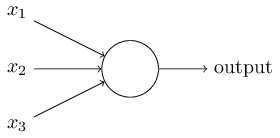
\includegraphics{perceptron.pdf}
	\caption{感知器模型}
	\label{perceptron}
\end{figure}

如图//所示,感知器接收若干个二进制输入$x_1, x_2, x_3, ...$并输出一个二进制结果。Rosenblatt 提出了一种计算感知机输出值的简易准则,他引入“权重(weight)”
的概念,用实数$w_1, w_2,...$来表示每个输入的重要性。最后神经元的输出,0 或者 1,是由加权和 $\sum_j w_{j}x_{j}$是否小于某个门限值决定的。和
权重一样,门限值也是神经元的一个实数参数。以上准则可由下面的公式\ref{eqn:perceptron}表示:
\begin{equation}
\label{eqn:perceptron}
output = \left\{ \begin{array} { l l } { 0 } & { \text { if } \sum _ { j } w _ { j } x _ { j } \leq \text { 门限 } } \\ { 1 } & { \text { if } \sum _ { j } w _ { j } x _ { j } > \text { 门限 } } \end{array} \right.
\end{equation}

以上就是感知器的简单数学模型。可以把感知器看成是一种对输入特征进行加权并输出决策的设备。可以结合实际举一个简单的例子。假如某人要决定周末是否
外出游玩,那么影响他决策的因素就可能是以下三个方面:

1. 天气是否晴好?

2. 是否有同伴陪同?

3. 游玩地点是否在地铁站附近?

我们可以用变量$x_1, x_2, x_3$来表征这三个二进制影响因素,比如$x_1 = 1$表示天气晴好,$x_2 = 1$表示有同伴陪同,$x_3 = 1$表示目标地点在地铁站
附近。

以上三个影响因素对最后的决定的影响程度是不一样的,这就需要对每个影响因素设置一个权重。假如天气是最关键的决定因素,在天气坏的情况下仍然出门的可能性很小,
那么就可将$x_1$对应的权重设置为$w_1=6$,其余两个影响因素的权重都设置为$w_2=1, w_3=1$。现在假如我们把门限值设置为 3,那么在天气坏的情况下,无论
其他两个因素是什么样的,最后的加权和都不会超过 3,从而做出周末不外出游玩这个决定。

通过设置不同的权重和门限,可得到不同的决策模型。比如将门限值降低可增加外出游玩的可能性,将是否有同伴陪同的权重提高可增加同伴对外出游玩与否的影响程度。

显然以上的感知器模型并不能完全体现人类决策的复杂性而只是一个简单的示例。通过堆叠多层感知器,可得到做出更加微妙决策的感知器网络。

\begin{figure}[h]
	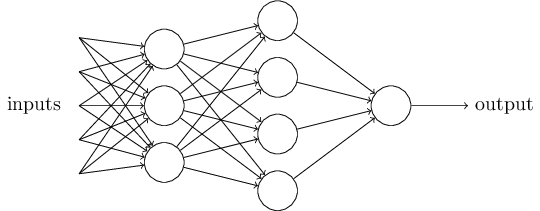
\includegraphics{layeredperceptron.pdf}
	\caption{多层感知器模型}
	\label{layeredperceptron}
\end{figure}

如图\ref{layeredperceptron},第一层感知器一共做出三项简单决策,这三项决策又接着输入到第二层的两个感知器得出两个更进一步的决策,最后这两个决策又输入到最后一个感知器得到
最后的决策。这种级联方式可以让后面的感知器得出比前面的感知器更抽象的结果,从而解决更加复杂的决策问题。

通过引入“偏置(bias)”$b$,公式\ref{eqn:perceptron}也可以改写为公式\ref{eqn:perceptronbias}:
\begin{equation}
	\label{eqn:perceptronbias}
output = \left\{ \begin{array} { l l } { 0 } & { \text { if } w \cdot x + b \leq 0 } \\ { 1 } & { \text { if } w \cdot x + b > 0 } \end{array} \right.
\end{equation}

偏置的概念可理解为输出 1 的容易程度。从生物学的角度也可说成神经元达到激发态的容易程度。偏置的引入可简化后面的公式表示。

\section{激活函数}
本节所介绍的激活函数的引入是为了使人工神经网络中感知器的权重和偏置的自动化训练成为可能。如果我们想通过调整感知器参数从而使网络的整体
表现满足某种特定需求,那么对感知器参数的微小改动必须也对应输出的微小改动,即稍稍改变权重和偏置不会导致输出的剧烈变化。前面的感知器模型只能输出0和1
两种结果,显然不能满足输出缓慢变化的特征。为了得到满足这种特征的感知器,需要对上节感知器模型做出修改,在输出时应用激活函数 $f$:
\begin{equation}
	\label{eqn:sigmoid}
	\sigma ( z ) \equiv \frac { 1 } { 1 + e ^ { - z } }
\end{equation}

即,对于输入$x_1, x_2, ...$,权重$w_1, w_2, w_3,...$ 和权重 $b$,sigmoid 神经元的输出是:
\begin{equation}
	\label{eqn:sigmoidoutput}
	\frac { 1 } { 1 + \exp \left( - \sum _ { j } w _ { j } x _ { j } - b \right) }
\end{equation}
从图\ref{sigmoid_step}可以看出,本质上 sigmoid 函数是阶跃函数的平滑版本,这也说明了为什么 sigmoid 激活函数的引入可以解决输出剧烈变化的问题。

\begin{figure}[htbp]
	\subfigure[]{
		\label{sigmoid}
		\includegraphics{sigmoid.pdf}}
	\subfigure[]{
		\label{step}
		\includegraphics{step.pdf}}
	\caption{Sigmoid 与阶跃函数对比图}
	\label{sigmoid_step}
\end{figure}

$\sigma$ 函数的重要性在于其平滑性,而与其具体的形状并没有太大的关系,$\sigma$ 的平滑度意味着权重中的微小变化
$\Delta w_j$ 和偏置中的 $\Delta w_j$ 将在神经元的输出中产生小的变化 $\Delta output$。
 事实上,微积分告诉我们 $\Delta output$ 很接近:
\begin{equation}
	\label{eqn:sigmoiddelta}
	\Delta \mathrm { output } \approx \sum _ { j } \frac { \partial \mathrm { output } } { \partial w _ { j } } \Delta w _ { j } + \frac { \partial \text { output } } { \partial b } \Delta b
\end{equation}

$\sigma$ 函数并不是唯一的激活函数形式,常用的激活函数还有 ReLU 激活函数。此函数是一个分段线性函数:
\begin{equation}
	\label{eqn:relu}
	\operatorname { ReLU } ( x ) = \left\{ \begin{array} { l l } { x } & { \text { if } x > 0 } \\ { 0 } & { \text { if } x \leq 0 } \end{array} \right.
\end{equation}

函数图像是:
\begin{figure}[htbp]
	\includegraphics{relu.pdf}
	\caption{ReLU 激活函数图像}
	\label{relu}
\end{figure}

从公式\ref{eqn:relu}和图\ref{relu}可以观察到 ReLU 函数把所有的负值都变为0,而正值线性变化,这种操作叫做单侧抑制。
尤其体现在深度神经网络模型(如CNN)中,当模型增加N层之后,理论上 ReLU 神经元的激活率将降低2的N次方倍。
相对于 sigmoid 函数,ReLU 能更好地实现网络模型的稀疏性,同时也符合近年来神经科学对神经元工作稀疏性的研究【引用】,同时 ReLu 在
正区间梯度总是为定值的特性也有利于避免梯度消失问题。

\section{神经网络结构}
单个感知器或者说人工神经元只是生物神经细胞的近似理
想化实现,功能更加简单。要想模仿人类的神经系统的推理运算功能,需要多个人工神经的协调配合实现高阶的抽象能力
并完成复杂的功能。通过特定的连接或信息传递方式进行配合的神经元可以看作是一个网络,我们称之为人工神经网络。

\begin{figure}[htbp]
	\includegraphics{ann_structure.pdf}
	\caption{神经网络一般结构}
	\label{ann_structure}
\end{figure}

图\ref{ann_structure}给出了人工神经网络的一般结构。人工神经网络一般由多层感知器级联而成。第一层感知器,也就是图中的最左边那层称为
输入层,它的作用是将输入数据传递到网络中。最后一层感知器被称为输出层,也就是图中的最右那层,用来得到网络的计算结果。
而输入层和输出层之间的各层统称为隐含层(hidden layer),隐含的意思是这些神经元处于神经网络内部,不与外部直接进行
信息交换。上图中的隐含层层数为 2,不过隐含层的层数也可以是任意正整数。历史上这类简单的多层神经网络也被成为多层感知机
(multilayer perceptrons)。

目前所提到的神经网络结构都是不包含反馈结构的,即所有网络层的输入都来自于上一层的输出,这种网络结构被称为前馈神经网络
(feedforward neural networks)。另外一种神经网络类型包含循环结构,即存在某些层的输出又作为前面网络层输入的情况,这种
网络结构统称为循环神经网络(recurrent neural networks)。循环神经网络在时序信号的处理,如语音识别领域,取得了良好
的效果。

\begin{figure}[htbp]
	\includegraphics{rnn_structure.pdf}
	\caption{循环神经网络}
	\label{rnn_structure}
\end{figure}

前馈神经网络是应用最广泛的神经网络模型,性能良好,也比较易于实现与调参,本文后面章节在处理探地雷达信号目标识别问题
时使用的卷积神经网络也属于前馈神经网络的一种。

\section{反向传播算法}
在将神经网络应用到分类和回归任务时,神经网络的预测性能由每层各神经元的权重和偏置组成的参数矩阵决定。神经网络的训练过程
即用特定的优化方法调整参数矩阵,使神经网络能特定的输入产生我们期望的输出。

对于一个前馈神经网络,我们使用下面的方法标记各参量。用 $L$:表示神经网络的层数;用$m^{(l)}$表示第$l$层神经元的个数;用
$f_l ()$ 表示$l$层的激活函数;$W ^ { ( l ) } \in \mathbb { R } ^ { m ^ { ( l ) } \times m ^ { l - 1 } }$ 用来表示
$l-1$ 层到 $l$ 层的权重矩阵;$\mathbf { b } ^ { ( l ) } \in \mathbb { R } ^ { m ^ { l } }$ 表示偏置矩阵;
$\mathbf { z } ^ { ( l ) } \in \mathbb { R } ^ { m ^ { l } }$ 表示$l$层神经元的净输入;$\mathbf { a } ^ { ( l ) } \in \mathbb { R } ^ { m ^ { l } }$
表示$l$层神经元的输出。

则我们可以用以下公式描述信息在前馈神经网络中的传播过程:
\begin{equation}
	\label{eqn:qiankuichuanbo1}
	\mathbf { z } ^ { ( l ) } = W ^ { ( l ) } \cdot \mathbf { a } ^ { ( l - 1 ) } + \mathbf { b } ^ { ( l ) }
\end{equation}
\begin{equation}
	\label{eqn:qiankuichuanbo2}
	\mathbf { a } ^ { ( l ) } = f _ { l } \left( \mathbf { z } ^ { ( l ) } \right)
\end{equation}

\ref{eqn:qiankuichuanbo1} 与 \ref{eqn:qiankuichuanbo2} 也可以合并为:
\begin{equation}
	\label{eqn:qiankuichuanbo3}
	\mathbf { z } ^ { ( l ) } = W ^ { ( l ) } \cdot f _ { l - 1 } \left( \mathbf { z } ^ { ( l - 1 ) } \right) + \mathbf { b } ^ { ( l ) }
\end{equation}

或者:
\begin{equation}
	\label{eqn:qiankuichuanbo4}
	\mathbf { a } ^ { ( l ) } = f _ { l } \left( W ^ { ( l ) } \cdot \mathbf { a } ^ { ( l - 1 ) } + \mathbf { b } ^ { ( l ) } \right)
\end{equation}

由此可以得到数据在更层传播的路径 \ref{eqn:qiankuichuanbo5},将向量 $\mathbf{x}$ 作为第 1 层的输入经过逐次传播后可得到将整个网络看成一个整体的
复合函数 $\phi(\mathbf{x} ; W, \mathbf{b})$
,其中 $L$ 表示总层数。
\begin{equation}
	\label{eqn:qiankuichuanbo5}
	\mathbf{x}=\mathbf{a}^{(0)} \rightarrow \mathbf{z}^{(1)} \rightarrow \mathbf{a}^{(1)} \rightarrow \mathbf{z}^{(2)} \rightarrow \cdots \rightarrow \mathbf{a}^{(L-1)} \rightarrow \mathbf{z}^{(L)} \rightarrow \mathbf{a}^{(L)}=\varphi(\mathbf{x} ; W, \mathbf{b}) )
\end{equation}

1989 年,Cybenko 等人的研究证明【引用】,上述前馈神经网络所表征的 $\phi(\mathbf{x} ; W, \mathbf{b})$ 函数在隐含神经元足够多的情况下,可以无限
你和任意的连续非线性函数。这说明神经网络具有通用近似能力,这也是用神经网络来解决机器学习问题的理论基础。

对于分类问题,还需要将 $\phi$ 函数作为某种分类器的输入,从而得到每种类别的概率。
\begin{equation} 
\hat{y}=g(\varphi(\mathbf{x}), \theta)
\end{equation}
其中,$\hat{y}$ 为每类的概率输出,$\theta$ 为分类器的参数,$g$ 为分类器。

对于多分类问题,常用的分类器为 Softmax 分类器。对于具有$N$个分类的多分类问题,式\ref{eqn:softmax}给出了 softmax 函数的定义。softmax 函数可以
将一组 $\phi$ 给出的输出转化为一组总和为1的概率,并且不影响转化前的大小相对关系。通过分类器的归一化之后的概率输出便可得出最可能的预测,因此分类器
基本上位于网络的最后一层。
\begin{equation} 
\label{eqn:softmax}
\operatorname{softmax}\left(s_{i}\right)=\frac{e^{s_{i}}}{\sum_{j=1}^{N} e^{s_{j}}} \quad(i=1, \cdots, N)
\end{equation}

上面说明了数据在前馈神经网络中正向传播的过程。为了使神经网络得到可靠的预测结果,需要对网络的参数,包括各层的权值和偏置,进行训练。训练一般采用
梯度下降算法,梯度下降时需要一个评估模型预测性能的损失函数。损失函数一般由模型预测结构和真实结构的交叉熵计算得出。交叉熵由式\ref{eqn:cross_entrophy}定义。
\begin{equation}
\label{eqn:cross_entrophy} 
\mathcal{L}(\mathbf{y}, \hat{\mathbf{y}})=-\mathbf{y}^{\mathrm{T}} \log \hat{\mathbf{y}}
 \end{equation}
其中$\mathbf{y}$与$\hat{\mathbf{y}}$分别表示实际标签与预测结果。

在交叉熵的基础上还可以定义风险函数:
\begin{equation} 
\mathcal{R}(W, \mathbf{b})=\frac{1}{N} \sum_{n=1}^{N} \mathcal{L}\left(\mathbf{y}^{(n)}, \hat{\mathbf{y}}^{(n)}\right)+\frac{1}{2} \lambda\|W\|_{F}^{2}
\end{equation}
\begin{equation} 
=\frac{1}{N} \sum_{n=1}^{N} \mathcal{L}\left(\mathbf{y}^{(n)}, \hat{\mathbf{y}}^{(n)}\right)+\frac{1}{2} \lambda\|W\|_{F}^{2}
\end{equation}
其中$\mathbf{W}$和$\mathbf{b}$分别表示网络中的权重和偏置;其中$\|W\|_{F}^{2}$为了防止过拟合现象而引入的正则化项;$\lambda$是为正数的参数。
这里的正则化项一般由Frobenius范数(式\ref{eqn:frobenius})给出:
\begin{equation} 
\label{eqn:frobenius}
\|W\|_{F}^{2}=\sum_{l=1}^{L} \sum_{i=1}^{m^{(l)}} \sum_{j=1}^{(l-1)}\left(W_{i j}^{(l)}\right)^{2}
\end{equation}

对模型的训练过程即调整模型参数使得风险函数最小的过程。按照梯度下降原理,每次迭代过程中第$l$层
的参数更新公式为:
\begin{equation} 
\begin{aligned} W^{(l)} & \leftarrow W^{(l)}-\alpha \frac{\partial \mathcal{R}(W, \mathbf{b})}{\partial W^{(l)}} \\ &=W^{(l)}-\alpha\left(\frac{1}{N} \sum_{n=1}^{N}\left(\frac{\partial \mathcal{L}\left(\mathbf{y}^{(n)}, \hat{\mathbf{y}}^{(n)}\right)}{\partial W^{(l)}}\right)+\lambda W^{(l)}\right) \\ \mathbf{b}^{(l)} & \leftarrow \mathbf{b}^{(l)}-\alpha \frac{\partial \mathcal{R}(W, \mathbf{b})}{\partial \mathbf{b}^{(l)}} \\ &=\mathbf{b}^{(l)}-\alpha\left(\frac{1}{N} \sum_{n=1}^{N} \frac{\partial \mathcal{L}\left(\mathbf{y}^{(n)}, \hat{\mathbf{y}}^{(n)}\right)}{\partial \mathbf{b}^{(l)}}\right) \end{aligned}
\end{equation}
式中的$\alpha$代表学习率。

使用梯度下降对神经网络参数进行优化时需要计算损失函数$\mathcal{L}(\mathbf{y}, \hat{\mathbf{y}})$关于每个参数的导数。
现在假设需要计算损失函数相对于$\mathbf{W}^{(l)}$和$\mathbf{b}^{(l)}$的偏导数。由于$\mathbf{W}^{(l)}$和$\mathbf{b}^{(l)}$
都是矩阵,如果要计算微分的话十分繁琐,所以可以先计算矩阵中某个元素的偏导数。根据求导法则,可得
\begin{equation} 
	\label{eqn:partial_l_partial_w}
	\frac{\partial \mathcal{L}(\mathbf{y}, \hat{\mathbf{y}})}{\partial W_{i j}^{(l)}}=\left(\frac{\partial \mathbf{z}^{(l)}}{\partial W_{i j}^{(l)}}\right)^{\mathrm{T}} \frac{\partial \mathcal{L}(\mathbf{y}, \hat{\mathbf{y}})}{\partial \mathbf{z}^{(l)}}
 \end{equation}
 \begin{equation}
	\label{eqn:partial_l_partial_b} 
 \frac{\partial \mathcal{L}(\mathbf{y}, \hat{\mathbf{y}})}{\partial \mathbf{b}^{(l)}}=\left(\frac{\partial \mathbf{z}^{(l)}}{\partial \mathbf{b}^{(l)}}\right)^{\mathrm{T}} \frac{\partial \mathcal{L}(\mathbf{y}, \hat{\mathbf{y}})}{\partial \mathbf{z}^{(l)}}
  \end{equation}

现在来计算$\frac{\partial \mathbf{z}^{(l)}}{\partial W_{i j}^{(l)}}$。
$\mathbf{z}^{(l)}$和$\partial W_{i j}^{(l)}$存在函数关系 $\mathbf{z}^{(l)}=W^{(l)} \mathbf{a}^{(l-1)}+\mathbf{b}^{(l)}$,所以
\begin{equation}
	\begin{aligned} 
\frac{\partial \mathbf{z}^{(l)}}{\partial W_{i j}^{(l)}}&=\frac{\partial\left(W^{(l)} \mathbf{a}^{(l-1)}+\mathbf{b}^{(l)}\right)}{\partial W_{i j}^{(l)}}\\
&=\left[ \begin{array}{c}{\frac{\partial\left(W_{1 :}^{(l)} \mathbf{a}^{(l-1)}+\mathbf{b}^{(l)}\right)}{\partial W_{i j}^{(l)}}} \\
 {\vdots} \\ 
{\frac{\partial\left(W_{i :}^{(l)} \mathbf{a}^{(l-1)}+\mathbf{b}^{(l)}\right)}{\partial W_{i j}^{(l)}}} 
\\{\vdots}\\ 
{\frac{\partial\left(W_{m^{l}:}^{(l)} \mathbf{a}^{(l-1)}+\mathbf{b}^{(l)}\right)}
{\partial W_{i j}^{(l)}}}\end{array}\right]=\left[ \begin{array}{c}0\\{\vdots}\\a_j^{l-1}\\{\vdots}\\0\end{array}\right]\\
	&\triangleq \mathbb{I}_{i}\left(a_{j}^{(l-1)}\right)
\end{aligned}
\end{equation}
其中$W_{i :}^{(l)}$代表$W^{(l)}$的第$i$行。$\mathbb{I}_{i}\left(a_{j}^{(l-1)}\right)$代表第$i$行的值为
$a_{j}^{(l-1)}$的列向量。

下面来计算偏导数$\frac{\partial \mathbf{z}^{(l)}}{\partial \mathbf{b}^{(l)}}$。带入函数关系
$\mathbf{z}^{(l)}=W^{(l)} \mathbf{a}^{(l-1)}+\mathbf{b}^{(l)}$可得
\begin{equation} 
\frac{\partial \mathbf{z}^{(l)}}{\partial \mathbf{b}^{(l)}}=
\frac{\partial (W^{(l)} \mathbf{a}^{(l-1)}+\mathbf{b}^{(l)})}{\partial \mathbf{b}^{(l)}}
=\mathbf{I}_{m^{(l)}}
 \end{equation}
其中$\mathbf{I}_{m}(l)$为$m^{(l)}$阶单位矩阵。

最后我们来计算 $\frac{\partial \mathcal{L}(\mathbf{y}, \hat{\mathbf{y}})}{\partial \mathbf{z}^{(l)}}$。
这个偏导项通常被称为误差项,用来表征某层神经元对网络最后总误差的影响,我们把第$l$层的误差项记作$\delta(l)$。

根据$\mathbf{z}^{(l+1)}=W^{(l+1)} \mathbf{a}^{(l)}+\mathbf{b}^{(l+1)}$,对$\mathbf{a}$求导可得
\begin{equation} 
\frac{\partial \mathbf{z}^{(l+1)}}{\partial \mathbf{a}^{(l)}}=\left(W^{(l+1)}\right)^{\mathrm{T}}
 \end{equation}

用按位计算函数$f_{l}(\cdot)$表示$\mathbf{a}^{(l)}$可得
\begin{equation} 
\begin{aligned} \frac{\partial \mathbf{a}^{(l)}}{\partial \mathbf{z}^{(l)}} &=\frac{\partial f_{l}\left(\mathbf{z}^{(l)}\right)}{\partial \mathbf{z}^{(l)}} \\ &=\operatorname{diag}\left(f_{l}^{\prime}\left(\mathbf{z}^{(l)}\right)\right) \end{aligned}
 \end{equation}

根据求导法则,可得
\begin{equation} 
\label{eqn:back_propagation}
\begin{aligned} \delta^{(l)} & \triangleq \frac{\partial \mathcal{L}(\mathbf{y}, \hat{\mathbf{y}})}{\partial \mathbf{z}^{(l)}} \\ 
&=\frac{\partial \mathbf{a}^{(l)}}{\partial \mathbf{z}^{(l)}} \cdot \frac{\partial \mathbf{z}^{(l+1)}}{\partial \mathbf{a}^{(l+1)}} \cdot \frac{\partial \mathcal{L}(\mathbf{y}, \hat{\mathbf{y}})}{\partial \mathbf{z}(l+1)} \\ 
&=\operatorname{diag}\left(f_{l}^{\prime}\left(\mathbf{z}^{(l)}\right)\right) \cdot\left(W^{(l+1)}\right)^{\mathrm{T}} \cdot \delta^{(l+1)} \\ &=f_{l}^{\prime}\left(\mathbf{z}^{(l)}\right) \odot\left(\left(W^{(l+1)}\right)^{\mathrm{T}} \delta^{(l+1)}\right) \end{aligned}
\end{equation}
$\odot$是向量点积运算。

从式\ref{eqn:back_propagation}可以看出,后一层($l+1$层)的误差项决定了前一层($l$层)的误差项,这种误差沿着网络向上一层传播的
现象被称为反向传播。式\ref{eqn:back_propagation}的含义是后一层某个神经元的
误差项是后一层与这个神经元连接相连的神经元的误差项的权重和再乘上该神经元激活函数的梯度。

算得这三个偏导之后,公式\ref{eqn:partial_l_partial_w}可写成
\begin{equation} 
\frac{\partial \mathcal{L}(\mathbf{y}, \hat{\mathbf{y}})}{\partial W_{i j}^{(l)}}=\mathbb{I}_{i}\left(a_{j}^{(l-1)}\right)^{\mathrm{T}} \delta^{(l)}=\delta_{i}^{(l)} a_{j}^{(l-1)}
\end{equation}

因此,损失函数关于第$l$层权重的梯度是:
\begin{equation}
\label{eqn:gradient_w} 
\frac{\partial \mathcal{L}(\mathbf{y}, \hat{\mathbf{y}})}{\partial W^{(l)}}=\delta^{(l)}\left(\mathbf{a}^{(l-1)}\right)^{\mathrm{T}}
\end{equation}

损失函数关于第$l$层偏置的梯度为:
\begin{equation} 
\label{eqn:gradient_b}
\frac{\partial \mathcal{L}(\mathbf{y}, \hat{\mathbf{y}})}{\partial \mathbf{b}^{(l)}}=\delta^{(l)}
\end{equation}

因此,基于梯度下降和反向传播的神经网络训练算法可以归纳为:

1. 按从输入层到输出层的方向计算每一次的输入值$\mathbf{z^{(l)}}$和激活值$\mathbf{a^{(l)}}$; 

2. 按从输出层到输入层的方向,即传播方向的反方向计算误差项$\delta^{(l)}$; 

3. 按照式\ref{eqn:gradient_w}和式\ref{eqn:gradient_b}计算每层梯度,并根据梯度下降算法修改参数。

上述过程也可用伪代码来描述:
\begin{algorithm}[H]
	\KwData{训练集$\mathcal{D}=\left\{\left(\mathbf{x}^{(n)}, y^{(n)}\right)\right\}_{n=1}^{N}$,
	,验证集$\mathcal{V}$,学习率$\alpha$,正则化系数$\lambda$,
	层数$L$,第$l$层神经元数量$m^{(l)}$}
	随机初始化$W, \mathbf{b}$
	\While{
		错误率在验证集$\mathcal{V}$上持续下降
	}{
		随机打乱训练集中的样本;
		\For{
			$n = 1...N$
		}{
			选取训练样本($x^{(n)}, y^{(n)}$);

			从前往后计算输入值$\mathbf{z^{(l)}}$和激活值$\mathbf{a^{(l)}}$;
			
			计算误差项$\delta^{(l)}$;
			
			//计算每层导数
			
			$\forall l, \quad \frac{\partial \mathcal{L}\left(\mathbf{y}^{(n)}, \hat{\mathbf{y}}^{(n)}\right)}{\partial W^{(l)}}=\delta^{(l)}\left(\mathbf{a}^{(l-1)}\right)^{\mathrm{T}}$;
			
			$\forall l, \quad \frac{\partial \mathcal{L}\left(\mathbf{y}^{(n)}, \hat{\mathbf{y}}^{(n)}\right)}{\partial \mathbf{b}^{(l)}}=\delta^{(l)}$;
			
			//更新参数
			
			$W^{(l)} \leftarrow W^{(l)}-\alpha\left(\delta^{(l)}\left(\mathbf{a}^{(l-1)}\right)^{\mathrm{T}}+\lambda W^{(l)}\right)$;
			
			$\mathbf{b}^{(l)} \leftarrow \mathbf{b}^{(l)}-\alpha \delta^{(l)}$;
		}
	}
	\KwResult{权重和偏置$W,\mathbf{b}$}
	\caption{如何训练前馈神经网络}
   \end{algorithm}

\section{卷积神经网络}
上节所述传统的前馈神经网络一般采用全连接结构,即每层所有神经元的输出都与下层的每一个神经元相连,也就是每一个连接都尤其对应的权重参数。
随着网络层数的增加,网络模型中参数的数量也将急剧增加。这样将会导致两个问题,一是参数过多时导致模型训练时计算量过大训练效率低,二是过多的
参数很容易导致过拟合现象即网络模型不能正确提取数据中的关键特征而过分强调无关细节。

在图像处理领域,以上所述问题尤其严重,因为相比于一维信号,图片数据需要用二维矩阵来表示,数据量大。特别是在图片为彩色的情况下,对于红、绿、
蓝三个通道,都要对应一个二维矩阵,这又使数据成倍增加。另外,对于图像处理来说,有很多图像上的特征在局部都是不变的,如材质的纹理,人脸的五官等,如果使用
全连接网络则很难提取出这些局部的特征。

卷积神经网络就是针对以上两个问题提出的一种改进型神经网络结构,可以很好地应用于图像和视频的各种图像分类、物体识别、图像分割等问题。如前面章节
所述,探地雷达的回波信号是发射天线产生的电磁波脉冲在地层中的反射传到接收天线并通过接收机与采集板回传到PC端信号采集软件的一维实数信号,也就是
所谓的A扫。随着收发天线的移动,不断采集到的二维信号可组合形成 B 扫数据。B 扫数据在形式上可看成是一种图像数据,另外,雷达B扫图像中目标反射所
形成的类似于双曲线图像也有明显的局部化特征。虽然反射特征在整体B扫中的位置是不确定的,但是在每个反射特征的周围一块区域却存在着相似的特性。考虑到
以上特点,探地雷达数据符合卷积神经网络的应用领域和数据特点。本文后面章节将使用卷积神经网络对探地雷达目标识别问题进行处理,并与多层感知机的效果作
对比。

卷积神经网络是受生物学上感受野的机制而提出。感受野(receptive field)主要是指听觉、视觉等神经系统中一些神经元的特性,即神经元只接受其所支
配的刺激区域内的信号。在视觉神经系统中,视觉皮层中的神经细胞的输出依赖于视网膜上的光感受器。视网膜上的光感受器受刺激兴奋时,将神经冲动信
号传到视觉皮层,但不是所有视觉皮层中的神经元都会接受这些信号。一个神经元的感受野是指视网膜上的特定区域,只有这个区域内的刺激才能够激活该
神经元。
 
应用到机器学习领域。卷积神经网络主要用到了三个基本思想:局部感受野、权值共享和子采样。下面分别对这三种思想作阐述。

【局部感受野】

前面所述全连接前馈神经网络中,输入数据是一维的列向量。在卷积神经网络中输入是以多维的形式组织的.

和前面的网络类似,输入层数据也要连接到隐含层的神经元上,不过在卷积神经网络中,我们不会将每个输入都连接到每一个隐含层神经元上。
反之我们只会连接一小部分局部的输入数据。更精确地说,第一个隐含层的每一个神经元都会连接到输入神经元的一小块区域,比如说一个5x5
尺寸的正方形区域(共25个输入数据)。这种连接方式可由图\ref{perception_filed}来说明(图中没有画出所有的输入神经元到隐含层神经元的连接)。

\begin{figure}[htbp]
	\includegraphics{perception_field.pdf}
	\caption{卷积层连接方式}
	\label{perception_filed}
\end{figure}

上述正方形区域被称为隐含神经元的局部感受野。局部感受野可看成作用在输入数据上一个窗。每一个从局部感受野到对应隐含神经元的连接都包含一个
权重,另外这个对应的隐含神经元本身也会有一个偏置参量。

将代表局部感受野的正方形窗在输入数据上平移,同时平移对应的隐含神经元,我们即可将所有的局部感受野与隐含神经元连接起来。

【权值共享】

上面提到局部感受野到隐含神经元的每一个连接都包含一个权重,此权重可以由一个矩阵$\mathbf{w}$来表示,这个矩阵的尺寸与局部感受野的尺寸相同。
但是在这里有一个值得注意的地方,即对于卷积神经网络从输入层到隐含层的每一个权重矩阵都是共享的。权重共享的目的是解决局部特征的学习问题,
因为权重共享之后,在二维数据某一位置学习到的特征也可应用到二维数据的其他位置。应用权重共享之后,对于位置为$j$,$k$的隐含层神经元,其输出是:
\begin{equation} 
\label{eqn:cnn_hidden_neuron}
f\left(b+\sum_{l=0}^{k} \sum_{m=0}^{k} w_{l, m} a_{j+l, k+m}\right)
\end{equation}
其中,$f$ 是激活函数,$b$ 是共享的偏置,$w_{l,m}$ 是共享的权重矩阵,$a_{j+l,k+m}$ 是对应的感受野输入,$k$ 是感受野尺寸。同时这里还要指出,
式\ref{eqn:cnn_hidden_neuron}中的求和部分可能看成是一个二维卷积的过程,这也就是卷积神经网络名称的由来。

从输入层到隐含层的映射被称为特征映射,即此映射包含了从输入数据中学习到的一般特征。在卷积神经网络术语中,共享的权重矩阵
$\mathbf{w}$和偏置$b$又被称为“核”或者“滤波器”。一般情况下,单个特征映射无法满足抽象出数据中足够多二维特征的要求。
所以在实际应用中,输入层可以映射到多个并列的隐含层,其中每一个隐含层都对应一个独立的特征映射及滤波器。

【子采样】

上面包含卷积运算的隐含层叫做卷积层。除了卷积层,卷积神经网络中还包含汇聚层(pooling layer)。汇聚层的作用是对卷积层输出的数据做
简化,也就是子采样,它通常紧接着卷积层使用。汇聚层将隐含层的输出结果矩阵划分成一批重叠或者不重叠的区域,然后对每个区域应用汇聚函数
得到一个单个的值,这样做实质上就是把隐含层的输出结果尺寸减小,即子采样的过程。常用的汇聚函数有最大汇聚和平均汇聚两种,分别可以表示为
\ref{eqn:max_pooling} 与 \ref{eqn:mean_pooling}。
\begin{equation}
\label{eqn:max_pooling} 
Y_{m, n}^{d}=\max _{i \in R_{m, n}^{d}} x_{i}
\end{equation}
\begin{equation} 
\label{eqn:mean_pooling}
Y_{m, n}^{d}=\frac{1}{\left|R_{m, n}^{d}\right|} \sum_{i \in R_{m, n}^{d}} x_{i}
\end{equation}
使用汇聚层之后,可以在大大减少神经元的数量的同时使神经网络对于一些微小细节的改变保持不敏感性,避免过拟合的发生。

如图\ref{cnn_structure}所示,卷积层、汇聚层和全连接层一起构成一个典型的卷积神经网络。一个卷积块为连续M 个卷积层和b个汇聚层(M
通常设置为 2 $\sim$ 5, b为 0或 1)。一个卷积网络中可以堆叠 $N$ 个连续的卷积块,
然后在接着 K 个全连接层($N$ 的取值区间比较大,比如 1 $\sim$ 100或者更大;$K$
一般为0 ~ 2)。
\begin{figure}[h]
	\includegraphics{cnn_structure.pdf}
	\caption{卷积神经网络结构示意图}
	\label{cnn_structure}
\end{figure}

按照图\ref{cnn_structure}给出的连接方式,结合实际问题的特点,不断增加网络的层数,达到足够提取出数据中的抽象特征进行高准确度预测
的效果,这样的网络被称为深度卷积网络。由于深度卷积网络可以利用数据的二维结构,而且所需要训练的参数相对来说更少,因此它是目前深度
学习领域中应用较为广泛的网络结构。

\section{本章小结}
二十世纪五十年代提出的感知器是用来模拟生物体神经元活动的模型。感知器接收二进制
输入并输出一个二进制结果。感知器是组成人工神经网络的基础模块,通过多个感知器的
级联可用来表征复杂的决策过程。在原始感知器模型的基础上引入的激活函数是感知器中参数的自动化
训练成为可能,因为它使感知器的输出由离散的量变为连续的量,从而让感知器内部参数的微小变化
只会导致输出的微小改动。多个带有激活函数的感知器的互联可用来处理需要高阶抽象能力的问题,
这种互联的网络被称作人工神经网络。人工神经网络一般多层感知器级联而成。所有网络的输入都直接
来自于上一层输出的神经网络被称为前馈神经网络,若网络中存在循环结构则被称为循环神经网络。
神经网络的误差函数可在交叉熵的基础上定义,误差函数用来在采用梯度下降算法优化网络参数时
评估模型预测性能。反向传播算法使计算误差函数对于各层权值和偏置的梯度称为可能,这是梯度下降法
求解最优化问题时的关键步骤。卷积网络是近年来火热的解决图像等二维数据识别问题的有效网络结构,
其结构主要特点是局部感受野、子采样和权值共享。卷积神经网络特别适合解决雷达B扫图像的相关识别问题。

\chapter{地下探测FDTD仿真技术研究}
本章的主要是内容是探地雷达应用到地下目标探测时的仿真技术。在将深度学习相关技术,特别是深度卷积神经网络
技术应用到探地雷达地下目标识别时需要提供大量的训练与测试数据用于神经网络的性能调优、结构调整、参数选择等等
过程。由于电磁仿真所得的数据具有目标位置明确模型参数已知的特点,在进行神经网络建模时就有了明确的参考
依据,可以验证网络的预测正确性和性能。另外,数值仿真也有数据获取简单,能用批量得到不同目标参数的B扫数据的特点。
因此,在将深度学习技术应用到实际实验数据之前,先在大量仿真数据上进行
初始研究是有重要意义的,这将为后面的工作提供良好的准备。

目前在探地雷达数值仿真领域,由于其原理简单、容易并行加速的特点,最常用的且最成熟的方法为时域有限差分(FDTD)法(引用)。
常见的探地雷达数值仿真计算为了模型简便,通常采用简单几何模型、均匀介质、点源等近似方法,在普通应用时通常也能带来令人
足够满意的效果。
但是,由于本文进行探地雷达数值仿真的目的是为深度学习目标识别技术的研究提供训练数据,需要仿真所得的数据尽量接近实际数据的特点,
这样才能对网络的实际性能做可信的评判,如果仿真模型过于理想化则生成的B扫数据会具有明显的目标特征而在非目标位置呈现干净的
图像从而与实际实验中复杂的土壤和仪器环境所带来的诸多干扰和虚假目标不相吻合。具体来说,笔者在应用这些常规方法建模并进行数值仿真时发现
以下几个问题:
\begin{figure}[htbp]
	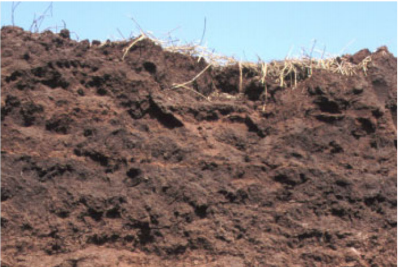
\includegraphics[width=0.8\textwidth]{soil_profile.png}
	\caption{某地土壤切面图(资料来自美国农业部官网)}
	\label{soil_profile}
\end{figure}

1. 简单几何模型不能模拟土壤表面复杂的起伏特征。如图\ref{soil_profile}所示,真实土壤表面呈现凹凸不平的起伏特征,这将会在雷达回波中
引入相当程度的抖动等干扰,而常规仿真方法中使用的标准长方体模型的边界是完美的平面,不能代表实际土壤的形态。所以需要研究土壤表面起伏
的数据特征并构想相关的模型生成算法。

2. 均匀介质模型不能模拟土壤中介质的随机分布特征。观察图\ref{soil_profile}中的土壤剖面可看到不均匀的土壤颗粒分布特征,土壤中介质
的不均匀分布必将导致雷达波传播过程中的路径和散射特征的改变,从来对雷达B扫图像引起干扰。常规方法中所使用的均匀介质,除了在不同介质的
相交面这样的介质参数突变的位置,对雷达波不会产生任何扭曲和路径改变,产生的数据过于理想化。因此需要研究土壤介质的构成模型和分布特点
并提供相应的建模算法以模拟真实土壤的介质形态。

3. 点源模型不能模拟近场状态时天线的传输特征。常规仿真方法通常将探地雷达天线近似为单个网格的点源模型,但是由于本文所研究的目标识别问题
中目标和天线的距离较近,且该距离接近天线的工作频率波长,因此此时天线的传输特征对雷达B扫图像将产生可见的影响,不符合尽量获取拟真数据
的目标,因此继续使用常规方法中的点源模型将不是理想的选择。

本章主要内容安排为:1. 介绍FDTD仿真的基本原理和开源数值仿真平台gprMax;2. 针对模拟土壤表面复杂起伏特征和介质随机
分布特征的问题,基于土壤介质参数半经验模型和FFT分形数据生成算法形成真实土壤模型构建算法;3. 针对模拟天线传输特征的问题,
研究将真实天线几何模型内置到FDTD网格的方法。4. 综合前面几节的结果,批量得到拟真雷达B扫图像。
\section{仿真方法与计算平台}
常用的电磁仿真方法有矩量法、有限元法和FDTD法。其中有限元法的理论基础是变分和插值,适用于求解各类微分方程问题,特别是物理场的求解问题;
矩量法的求解目标是代数方程组,这些方程组由待求解积分或微分方程转化而来;FDTD法以差分原理为基础,将麦克斯韦方程中的微分算子通过差分近似。
FDTD法具有容易掌握,直观简洁的特点,其计算迭代方程可由麦克斯韦方程直接导出而且不需要进行其他复杂的推导过程,另外由于其将空间划分为均匀的
立方体网格,所以也特别适合复杂模型的程序化生成,特别是本章要解决的土壤与天线建模问题。
\subsection{FDTD方法基本原理}
\begin{figure}[htbp]
	\includegraphics{yee_cube.pdf}
	\caption{FDTD网格示意图}
	\label{yee_cube}
\end{figure}

FDTD法的基本思想是将计算空间离散为一个一个的矩形网格(图\ref{yee_cube}),然后再将磁场与电场矢量分布到这些网格上,其中磁场位于每个立方体各个面的重心处且
垂直于该表面,电常位于各条边中心且与其平行。将$\mathbf{E}_x$、$\mathbf{E}_y$、$\mathbf{E}_z$、
$\mathbf{H}_x$、$\mathbf{H}_y$、$\mathbf{H}_z$六个分量以Maxwell方程组联系起来,即可得到:
\begin{equation} 
\varepsilon \frac{\partial E_{x}}{\partial t}=\frac{\partial H_{z}}{\partial y}-\frac{\partial H_{y}}{\partial z}-\sigma E_{x}
\label{eqn:maxwell_1} 
\end{equation}
 \begin{equation} 
 \varepsilon \frac{\partial E_{y}}{\partial t}=\frac{\partial H_{x}}{\partial z}-\frac{\partial H_{z}}{\partial x}-\sigma E_{y}
  \end{equation}
  \begin{equation} 
  \varepsilon \frac{\partial E_{z}}{\partial t}=\frac{\partial H_{y}}{\partial x}-\frac{\partial H_{x}}{\partial y}-\sigma E_{z}
   \end{equation}
   \begin{equation} 
\mu \frac{\partial H_{x}}{\partial t}=\frac{\partial E_{y}}{\partial z}-\frac{\partial E_{z}}{\partial y}
 \end{equation}
 \begin{equation} 
\mu \frac{\partial H_{y}}{\partial t}=\frac{\partial E_{z}}{\partial x}-\frac{\partial E_{x}}{\partial z}
 \end{equation}
 \begin{equation} 
	\label{eqn:maxwell_6}
\mu \frac{\partial H_{z}}{\partial t}=\frac{\partial E_{x}}{\partial y}-\frac{\partial E_{y}}{\partial x}
 \end{equation}

 以上6个分量均可由对于三个空间方向以及时间方向的偏导数,也就是对于$x, y, z, t$的偏导数都可以以下中心差分公式
 近似表示:
 \begin{equation} 
 \frac{\partial f(\xi)}{\partial \xi}=\frac{\partial f(\xi+\Delta \xi / 2)}{\partial \xi}-\frac{\partial f(\xi-\Delta \xi / 2)}{\partial \xi}
  \end{equation}

代入式(\ref{eqn:maxwell_1}) \textasciitilde (\ref{eqn:maxwell_6})即可得到Maxwell方程的离散形式:
\begin{equation} 
\begin{array}{l}{E_{x}^{n+1}\left(i+\frac{1}{2}, j, k\right)=\left(\frac{2 \varepsilon-\sigma \Delta t}{2 \varepsilon+\sigma \Delta t}\right) E_{x}^{n}\left(i+\frac{1}{2}, j, k\right)+\left(\frac{2 \Delta t}{2 \varepsilon+\sigma \Delta t}\right)\{ } \\ {\frac{1}{\Delta y}\left[H_{z}^{n+\frac{1}{2}}\left(i+\frac{1}{2}, j+\frac{1}{2}, k\right)-H_{z}^{n+\frac{1}{2}}\left(i+\frac{1}{2}, j-\frac{1}{2}, k\right)\right]-} \\ {\frac{1}{\Delta z}\left[H_{y}^{n+\frac{1}{2}}\left(i+\frac{1}{2}, j, k+\frac{1}{2}\right)-H_{y}^{n+\frac{1}{2}}\left(i+\frac{1}{2}, j, k-\frac{1}{2}\right)\right]}\end{array}
 \end{equation}
 \begin{equation} 
\begin{array}{l}{E_{y}^{n+1}\left(i, j+\frac{1}{2}, k\right)=\left(\frac{2 \varepsilon-\sigma \Delta t}{2 \varepsilon+\sigma \Delta t}\right) E_{y}^{n}\left(i, j+\frac{1}{2}, k\right)+\left(\frac{2 \Delta t}{2 \varepsilon+\sigma \Delta t}\right)\{ } \\ {\frac{1}{\Delta z}\left[H_{x}^{n+\frac{1}{2}}\left(i, j+\frac{1}{2}, k+\frac{1}{2}\right)-H_{x}^{n+\frac{1}{2}}\left(i+\frac{1}{2}, j, k-\frac{1}{2}\right)\right]-} \\ {\frac{1}{\Delta x}\left[H_{z}^{n+\frac{1}{2}}\left(i+\frac{1}{2}, j+\frac{1}{2}, k\right)-H_{z}^{n+\frac{1}{2}}\left(i-\frac{1}{2}, j+\frac{1}{2}, k\right)\right]}\end{array}
 \end{equation}
 \begin{equation} 
\begin{array}{l}{E_{z}^{n+1}\left(i, j, k+\frac{1}{2}\right)=\left(\frac{2 \varepsilon-\sigma \Delta t}{2 \varepsilon+\sigma \Delta t}\right) E_{z}^{n}\left(i, j+\frac{1}{2}, k\right)+\left(\frac{2 \Delta t}{2 \varepsilon+\sigma \Delta t}\right)\{ } \\ {\frac{1}{\Delta x}\left[H_{y}^{n+\frac{1}{2}}\left(i+\frac{1}{2}, j, k+\frac{1}{2}\right)-H_{y}^{n+\frac{1}{2}}\left(i-\frac{1}{2}, j, k+\frac{1}{2}\right)\right]-} \\ {\frac{1}{\Delta y}\left[H_{x}^{n+\frac{1}{2}}\left(i, j+\frac{1}{2}, k+\frac{1}{2}\right)-H_{x}^{n+\frac{1}{2}}\left(i, j-\frac{1}{2}, k+\frac{1}{2}\right)\right]}\end{array}
 \end{equation}
 \begin{equation} 
\begin{array}{l}{H_{x}^{n+\frac{1}{2}}\left(i, j+\frac{1}{2}, k+\frac{1}{2}\right)=\left(\frac{2 \mu-\sigma \Delta t}{2 \mu+\sigma \Delta t}\right) H_{x}^{n-\frac{1}{2}}\left(i, j+\frac{1}{2}, k+\frac{1}{2}\right)-} \\ {\left(\frac{2 \Delta t}{2 \mu+\sigma \Delta t}\right)\left\{\frac{1}{\Delta y}\left[E_{z}^{n}\left(i, j+1, k+\frac{1}{2}\right)-E_{z}^{n}\left(i, j, k+\frac{1}{2}\right)\right]-\right.} \\ {\frac{1}{\Delta z}\left[E_{y}^{n}\left(i, j+\frac{1}{2}, k+1\right)-E_{y}^{n}\left(i, j+\frac{1}{2}, k\right)\right]}\end{array}
 \end{equation}
 \begin{equation} 
\begin{array}{l}{H_{y}^{n+\frac{1}{2}}\left(i+\frac{1}{2}, j, k+\frac{1}{2}\right)=\left(\frac{2 \mu-\sigma \Delta t}{2 \mu+\sigma \Delta t}\right) H_{y}^{n-\frac{1}{2}}\left(i+\frac{1}{2}, j, k+\frac{1}{2}\right)-} \\ {\left(\frac{2 \Delta t}{2 \mu+\sigma \Delta t}\right)\left\{\frac{1}{\Delta z}\left[E_{x}^{n}\left(i+\frac{1}{2}, j, k+1\right)-E_{z}^{n}\left(i+\frac{1}{2}, j, k\right)\right]-\right.} \\ {\frac{1}{\Delta x}\left[E_{z}^{n}\left(i+1, j, k+\frac{1}{2}\right)-E_{z}^{n}\left(i, j, k+\frac{1}{2}\right)\right]}\end{array}
 \end{equation}
 \begin{equation} 
\begin{array}{l}{H_{z}^{n+\frac{1}{2}}\left(i+\frac{1}{2}, j+\frac{1}{2}, k\right)=\left(\frac{2 \mu-\sigma \Delta t}{2 \mu+\sigma \Delta t}\right) H_{z}^{n-\frac{1}{2}}\left(i+\frac{1}{2}, j+\frac{1}{2}, k\right)-} \\ {\left(\frac{2 \Delta t}{2 \mu+\sigma \Delta t}\right)\left\{\frac{1}{\Delta x}\left[E_{y}^{n}\left(i+1, j+\frac{1}{2}, k\right)-E_{z}^{n}\left(i, j+\frac{1}{2}, k\right)\right]-\right.} \\ {\frac{1}{\Delta y}\left[E_{x}^{n}\left(i+\frac{1}{2}, j+1, k\right)-E_{x}^{n}\left(i+\frac{1}{2}, j, k\right)\right]}\end{array}
 \end{equation}

通过以上各式,在$t_0$时刻已知当前空间所有网格电场值的情况下,便可推得$t_0+{\Delta t}/2$时刻所有网格的磁场值,
再次步进${\Delta t}/2$时刻即又能得到$t_0+\Delta t$时刻的电场值。如此循环往复即可进行电磁波在自由空间与介质中
随时间传播的数值模拟结果。以上是FDTD方法的时间步进基本过程,关于其数值稳定性、误差分析和边界条件等细节在此便不再赘述。
\subsection{gprMax仿真平台}
通过上节的原理很容易自行编写可用的FDTD数值计算程序。笔者曾编写过基于C++与Matlab的三维FDTD仿真软件,两种程序均存在
一些难以克服的缺点。Matlab版由于Matlab强大的工程计算函数库和友好的界面很容易进行快速建模与结果可视化,但是其计算缓慢
,即使使用内置的并行接口其速度也难以达到本文的计算量需求。C语言版可生成高效原生代码,并且可借助并行计算程序包OpenMP在
实验室数值计算服务器上利用多核CPU的优势得到更快的计算速度。但是相对于Matlab版,C语言版却缺乏足够的灵活性,在复杂形体建模
方面需要书写大量的底层逻辑甚至需要用到专业的计算几何知识,此外C语言在数据的可视化方面也缺乏足够的工具,往往还是需要
借助其他工具进行数据处理。考虑到这些因素,本文采用英国爱丁堡大学团队开发的开源电磁仿真程序包gprMax
\citing{giannopoulos2005modelling, warren2016gprmax}作为FDTD计算引擎,并
利用其开源的优势进行大量的二次开发以满足本文中建模仿真的需要。

结合本文所研究问题的实际特点,gprMax 与C、Matlab以及其他常见商业软件相比以下显著优势:

计算速度快。最新版gprMax采用python语言开发,python作为一门脚本语言本身运行效率并不高,但是却可因为其胶水语言的特性
克服这一缺点。其主要加速途径主要有三方面:1. 可以对gprMax源码进行研究可发现内部其使用了Cython程序包。
Cython程序包可将普通的Python语句编译到C语言,从而解决解释性语言运行速度慢的问题。2. FDTD时间步进方程在计算时每个网格
场值只与上一时刻的场值有关,每个网格的计算是互相独立,因此可将计算空间划分为多个区域,并将每个区域分配给单独的CPU核心计算。
另外,在同时仿真多个模型时,还可以利用MPI调度集群内的多个CPU同时计算并汇总计算结果。3. 最新版本的gprMax开始支持基于英伟达
CUDA平台的GPU加速\citing{warren2019cuda},实测利用显卡的多核心矩阵运算能力可将计算时间缩短到之前的四十分之一左右。

极强的可扩展性。gprMax 的扩展能力使得用户可以很方便的定义属于自己的模型库和脚本化控制仿真的运行,特别适合需要建立复杂模型
与大量仿真的情形。在阅读其源码后也可以对内部计算流程进行修改和补充,比如改变仿真结果的保存格式。gprMax的扩展能力一方面来自于
其开源的特点,即所有代码可供用户阅读与修改,另一方面由于python语言在运行时不需要编译,用户所作的修改和自定义库可以和原有gprMax
程序无缝融合而不需要传统软件工程的构建流程,方便了使用者的自定义流程。

本章后面小节的建模与仿真充分利用了这两个优势。首先土壤天线建模和补充均以python用户模块的形式增强gprMax原有的功能。其次
仿真时均利用实验室高性能显卡实现了显著加速。

\section{拟真土壤模型}
本节所介绍的拟真土壤模型由两方面的理论组成,其一是土壤混合物的电磁参数模型,其二是地下介质分布和地形所蕴含的分形特征。
\subsection{拟真土壤模型原理}
1995年,Peplinski 等人提出一种模拟真实土壤电磁特性的半经验模型\citing{peplinski1995dielectric}。在此模型中,土壤由三种成分构成,分别是:
颗粒直径在0.05mm到2.0mm之间的沙土,颗粒直径在0.002mm到0.05mm之间的粉土,以及颗粒直径在0.002
以下的粘土。这三种成分的配比不同可表示不同的土壤类型,进而也影响到其电磁特性。同时,土壤中含水量也对
其电磁特性起重大影响。综合这些因素,土壤的复介电常数$\epsilon_m$由式(\ref{eqn:peplinskiall})给出。
\begin{equation} 
	\label{eqn:peplinskiall} 
	\begin{aligned} \epsilon_{m} &=\epsilon_{m}^{\prime}-j \epsilon_{m}^{\prime \prime} \\ 
\epsilon_{m}^{\prime} &=1.15 \left[1+\frac{\rho_{b}}{\rho_{s}}\left(\epsilon_{s}^{\alpha}\right)+m_{v}^{\beta^{\prime}} \epsilon_{f w}^{\alpha}-m_{v}\right]^{1 / \alpha} - 0.68\\ 
\epsilon_{m}^{\prime \prime} &=\left[m_{v}^{\beta^{\prime \prime}} \epsilon_{f w}^{\prime \prime \alpha}\right]^{1 / \alpha} \end{aligned}
\end{equation}

上式中,$\epsilon_{m}^{\prime}$ 与 $\epsilon_{m}^{\prime \prime}$分别是复介电常数
$\epsilon_m$的实部与虚部;$\rho_{b}$ 与 $\rho_{s}$分别是土壤的总密度和其中沙土成分
的密度(单位:$g/cm^3$);$\beta^\prime$与$\beta^{\prime \prime}$分别是与土壤构成
相关的常数,其表达式为\ref{eqn:soil_beta},其中$S$与$C$分别是沙土与粘土的构成比例
($0<S<1, 0<C<1$)。
\begin{equation} 
	\label{eqn:soil_beta}
	\begin{aligned}
\beta^{\prime}&=1.2748-0.519 S-0.152 C \\
\beta^{\prime \prime}&=1.33797-0.603 S-0.166 C
	\end{aligned}
\end{equation}

式(\ref{eqn:peplinskiall})中$\epsilon_{f w}^{\prime}$与$\epsilon_{f w}^{\prime \prime}$
分别是土壤中自由水的实部与虚部,其表达式由式(\ref{eqn:soil_water})给出。
\begin{equation} 
	\label{eqn:soil_water}
	\begin{aligned}
		\epsilon_{f w}^{\prime}&=\epsilon_{w \infty}+\frac{\epsilon_{w 0}-\epsilon_{w \infty}}{1+\left(2 \pi f \tau_{w}\right)^{2}} \\
		\epsilon_{f w}^{\prime \prime}&=\frac{2 \pi f \tau_{w}\left(\epsilon_{w 0}-\epsilon_{w \infty}\right)}{1+\left(2 \pi f \tau_{w}\right)^{2}}+\frac{\sigma_{\mathrm{eff}}}{2 \pi \epsilon_{0} f} \frac{\left(\rho_{s}-\rho_{b}\right)}{\rho_{s} m_{v}}
	\end{aligned}
\end{equation}
其中,$\epsilon_{w \infty}$是$\epsilon_{f w}^{\prime \prime}$在高频时的极限;$\tau_{w}$为自由水的
弛豫时间常数;$\epsilon_{w 0}$为水的静态相对介电常数,其值为80.1;$\sigma_{\mathrm{eff}}$为有效电导率
,由经验公式(\ref{eqn:soil_eff})给出。
\begin{equation}
	\label{eqn:soil_eff}
\sigma_{\mathrm{eff}}=0.0467+0.2204 \rho_{b}-0.4111 S+0.6614 C
\end{equation}

以上便是拟真土壤模型的基本原理,下面讨论如何将此模型应用到探地雷达FDTD仿真中。
按照式(\ref{eqn:peplinskiall}),在给定土壤构成比例$S$与$C$后,该土壤类型的电磁参量主要由含水量决定。
实际土壤中含水量的分布不是均匀的,因此可定义含水量的最小值与最大值分别为$m_{vmin}$与$m_{vmax}$。
将此含水量范围等距离取$n$个点并代入式(\ref{eqn:peplinskiall})便可得到一系列复介电常数
$\epsilon_i(i=1,2,3...n)$ 

得到组成土壤的介质列表之后,接下来了的问题便是考虑这些介质应该如何分布在FDTD三维网格中。文献
\cite{turcotte1997fractals}
指出地下空间内孔隙度含水量等特性的分布并不是完全随机的而是呈随机分形特征。因此可以利用分形生成算法安排前面得到的一系列介质在FDTD网格
中的分布从而达到对真实土壤较好的模拟效果。

分形在数学中是一种抽象的物体,用于描述自然界中存在的事物。人工分形通常在放大后能展现出相似的形状。 
分形也被称为扩展对称或展开对称。如果在每次放大后,
形状的重复是完全相同的,这被称为自相似。分形在不同的缩放级别上可以是近似相似的。 
分形也包有图像的细节重复自身的意味。一种效率较高的分形数据生成算法是以离散傅里叶变换为基础的。
其算法理论基础是具有分形特征的数据的离散傅里叶变换(DFT)上各频率
的系数$m_f$与频率$f$近似呈幂律关系,即:
\begin{equation}
m_f = \frac{C}{f^{\frac{-(2 D-7)}{2}}}
\end{equation}
其中$D$为分形维度,其值在1到3之间。

因此,可以用以下步骤生成生成复介电常数列表在土壤所在三维空间内FDTD网格的分形分布:

1. 对于尺寸为$x,y,z$的FDTD网格区域,生成相同大小的随机三维数据$\mathbf{A}$。

2. 对$\mathbf{A}$应用三维快速傅里叶变换算法,并将结果进行平移,使零频率处于三维数组
的中心。

3. 设$\mathbf{A}$的中心点的坐标为$(i_c,j_c,k_c)$,对于每一个数据点$\mathbf{A}(i,j,k)$
,计算其与中心点的模,即$L=\sqrt{(i - i_c)^2 + (j - j_c)^2 + (k - j_c)^2}$。

4. 应用公式 $\mathbf{A}(i,j,k) = \mathbf{A}(i,j,k) \frac{1}{L^{\frac{-(2 D-7)}{2}}}$。

5. 对$\mathbf{A}$进行逆傅里叶变换,并将结果归一化并量化为$1$到$n$的整数(对应土壤介质的个数),并在对应位置为FDTD网格的赋予相应
的介质参数。

要获得高度拟真的土壤模型,除了要考虑介质参数分布方面的特征,还要考虑到地形的特征。和土壤介质的分布一样,土壤表面起伏的
形态也符合分形的特征(图\ref{soil_profile})。

由于同样满足分形特征,土壤起伏表面也可由上述类似的方式生成,比较重要的变化是上面三维的数据变为二维的数据,
空间上的三维傅里叶变换变成平面上的二维傅里叶变换,但是其算法本质不变。其过程可描述为(定义土壤起伏程度为
$k$,分形维数为$D$:

1. 对于尺寸为$x,y$的FDTD网格区域(该区域为需要生成土壤起伏表面的土壤区域顶部所围成的二维区域),
生成相同大小的随机二维数据$\mathbf{A}$。

2. 对$\mathbf{A}$应用二维快速傅里叶变换算法,并将结果进行平移,使零频率处于二维数组
的中心。

3. 设$\mathbf{A}$的中心点的坐标为$(i_c,j_c)$,对于每一个数据点$\mathbf{A}(i,j)$
,计算其与中心点的模,即$L=\sqrt{(i - i_c)^2 + (j - j_c)^2}$。

4. 应用公式 
\begin{equation}
	\label{eqn:fractal_2d}
	\mathbf{A}(i,j) = \mathbf{A}(i,j) \frac{1}{L^{\frac{-(2 D-7)}{2}}}
\end{equation}

5. 对$\mathbf{A}$进行逆傅里叶变换,将所得结果归一化到$[-k,k]$范围内,此时$\mathbf{A}$即代表
土壤区域顶部对应的起伏程度,将此起伏程度数据应用于建模过程便可得到具有起伏表面的土壤模型。
\subsection{建模实例}
为了方便展示计算过程,这里对土壤起伏表面的生成过程做建模演示。图\ref{rough_surface}展示了上述土壤分形生成算法
中各步骤的计算结果,其中第一步中$x$和$y$的值皆为400,分形维数$D=1.5$。图\ref{rough_surface}(a)为原始随机矩阵,
在经过傅里叶变换后变为图\ref{rough_surface}(b),频域数据经过公式(\ref{eqn:fractal_2d})处理后能量集中到
低频区域,这一点可在图\ref{rough_surface}(c)看出来,其中能量由图中心的低频部分像周围的高频区域逐渐下降(图中的
颜色以对数尺度标出)。最后,如图\ref{rough_surface}{d}所示,恢复到时域的数据呈现类似于地形起伏的分形特征。
\begin{figure}[htbp]
	\subfigure[]{
		\label{rough_surface_a}
		\includegraphics{rough_surface_random.pdf}}
	\subfigure[]{
		\label{rough_surface_b}
		\includegraphics{rough_surface_fft.pdf}}
	\subfigure[]{
		\label{rough_surface_c}
		\includegraphics{rough_surface_fft_fractal.pdf}}
	\subfigure[]{
		\label{rough_surface_d}
		\includegraphics{rough_surface_fractal.pdf}
	}
	\caption{土壤起伏表面建模实例二维图。(a)随机二维数据;(b)随机数据的二维傅里叶变换;
	(c)应用公式(\ref{eqn:fractal_2d})后的结果;(d)最后生成的土壤起伏数据}
	\label{rough_surface}
\end{figure}

直观起见,图\ref{rough_surface_3d}给出了图\ref{rough_surface}(d)中数据的三维曲面图。设该曲面所代表的数据为
$\mathbf{A}_{fractal}$,且其最大值为$A_{max}$最小值为$A_{min}$。在将该结果应用到FDTD建模之前需要对其值的范围进行调整,若指定模型中该土壤表面高度值的
范围为$h_{min}$到$h_{max}$,则可根据下面的公式得出在FDTD模型中的实际表面高度。
\begin{equation}
	\mathbf{A}_{fractal} = \mathbf{A}_{fractal} \frac{h_{max} - h_{min}}{A_{max} - A_{min}} + 
		h_{min} - (\frac{h_{max} - h_{min}}{A_{max} - A_{min}}) h_{min}
\end{equation}
\begin{figure}[htbp]
	\includegraphics[]{rough_surface_fractal_3d.pdf}
	\caption[]{土壤起伏表面建模实例三维图}
	\label{rough_surface_3d}
\end{figure}

按照前述类似的过程也可以建立前述土壤介质分布模型,将此模型与起伏表面模型结合起来便得到完整的拟真土壤模型(图\ref{soil_model_3d})。


\begin{figure}[htbp]
	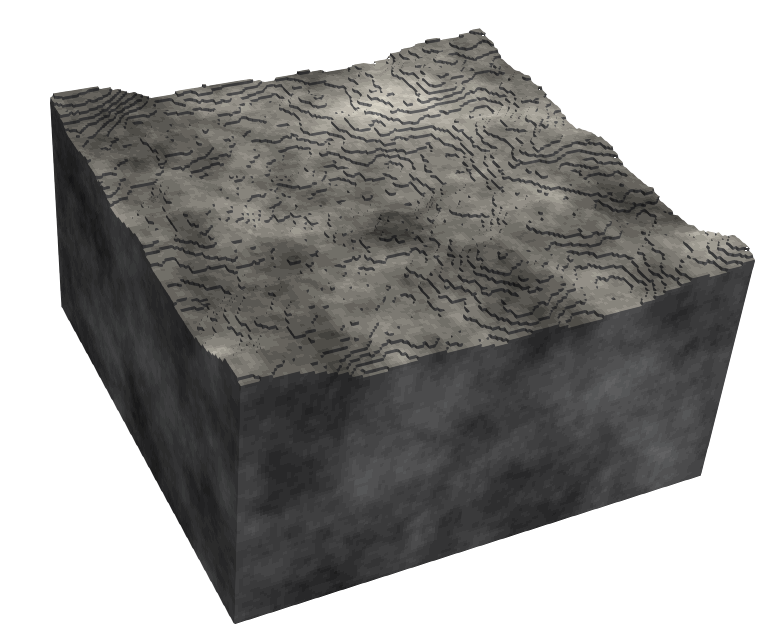
\includegraphics[width=0.8\textwidth]{soil_model_3d.png}
	\caption{拟真土壤模型建模示例}
	\label{soil_model_3d}
\end{figure}
\section{天线模型仿真}
探地雷达主要采用偶极子天线、蝶形天线、维瓦尔第天线等几种常用的天线类型。本节讨论FDTD网格中天线建模的方法,并给出建模实例。
\subsection{FDTD天线建模方法}
将天线模型置入FDTD过程中首先要考虑的问题是如何将实际的天线几何模型转化成离散的网格模型。对于结构较为简单的天线来说,如偶极子天线和蝶形天线,
天线的形状可由基本的几何形体构成,而这些基本的几何形体(三角形、矩形、长方体、球、圆柱等)在gprMax中都有对应的建模指令,因此处理起来较为方便,只需要
选择合适的网格尺寸将天线的结构用基本几何体描述出来即可。而对于包含复杂弧度的天线来说,直接用几何体无法拼接出想要的形状。在实践中笔者为了解决
这一问题提出了一套较为实用的解决方案。即先采用图像处理的方法先对天线设计稿进行预处理,标记出天线上金属板的范围。然后,根据FDTD网格尺寸的需要,将处理好的天线金属板图片进行离散化。
最后再次通过图像处理程序将图片中已标记的像素点的位置信息提取出来,然后在FDTD网格模型中使用边长正好等于网格尺寸的矩形板结构依次对应图片中的像素点位置信息。
这样便能将复杂的天线形状完美地移植到FDTD网格中。这一系列步骤将在后面的例子中演示。

其次,还需要考虑仿真过程中信号源加载的问题。在探地雷达实际工作过程中激励信号是由超宽带脉冲信号源产生并通过同轴电缆加载到收发天线的对应端口上。而在
FDTD仿真中,无法做到对信号源以及同轴电缆进行仿真。笔者通过数值实验发现,gprMax中带有内阻的点源可以很好的模拟同轴线端口并将激励信号通过天线金属板
辐射出去。这里还有两方面的问题需要注意。第一点是点源的极化方向需要与实际端口引出的连接到金属板的两个触电的方向一致,这样才能保证信号的传输方式和实际一样。
第二点,因为点源只占一个网格,因此为了让点源的电场同时加载到正负极板上,需要保证正负极板在加载位置只间隔一个网格,这样才不会出现点源与极板之间间隔有
自由空间的情况。

\subsection{仿真实例}
本节以笔者所在团队所设计的维瓦尔第天线\citing{guo2017ultrawideband}为例阐释复杂形状天线的建模过程。图\ref{vivaldi_design}分别给出了此天线的实物图
与设计稿。此天线尺寸为600mm x 450mm x 1mm,两片金属板分别位于基板的正反两面,基板由相对介电常数为3的绝缘材料构成,
馈电位置位于实物图设计稿底部中间位置。

图\ref{vivaldi_model_10mm}为天线设计稿经过图像处理并离散化后的结果,其中离散化的精度为10mm,这是兼顾了仿真精度与
仿真速度的选择。此图片为像素值只有0或1两种可能的二值化图形,因此很容易将其中的白色区域的坐标数据提取出来并将其导入gprMax的
FDTD网格中。

图\ref{vivaldi_fdtd_grid}是该天线金属部分在FDTD网格中的可视化图像。基板正反两面的金属板分别以不同颜色标出,两者所在的平面
相隔一个FDTD网格以便加载信号源。由于所用金属的电阻率很小,天线金属部分的介质设置为PEC(完美电导体)。基板部分按照实际所用
材料的参数将其相对介电常数设置为3。点源位于馈电位置在FDTD网格的对应位置,设置其内阻为$50\Omega$。
\begin{figure}[htbp]
	\subfigure[]{
		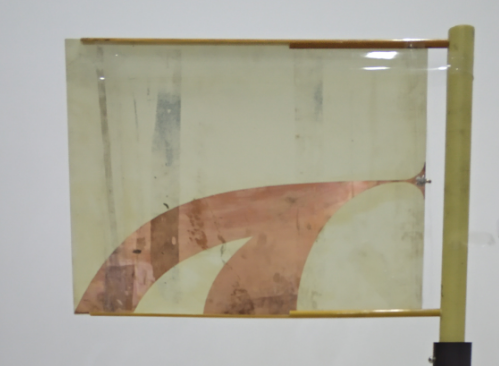
\includegraphics[width=0.4\textwidth]{vivaldi_real.png}
	}
	\subfigure[]{
		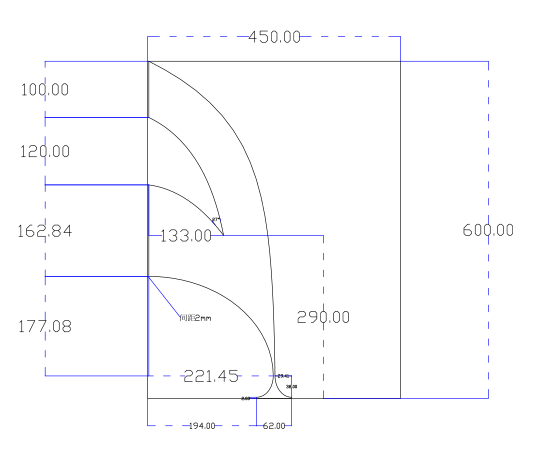
\includegraphics[width=0.4\textwidth]{vivaldi_design}
	}
	\caption[]{维瓦尔第天线。(a)实物图;(b)设计稿}
	\label{vivaldi_design}
\end{figure}

\begin{figure}[htbp]
	
\includegraphics[width=0.8\textwidth]{vivaldi_model_10mm.png}
	\caption[]{维瓦尔第天线几何模型离散化结果(网格尺寸10mm)}
	\label{vivaldi_model_10mm}
\end{figure}

\begin{figure}[htbp]
	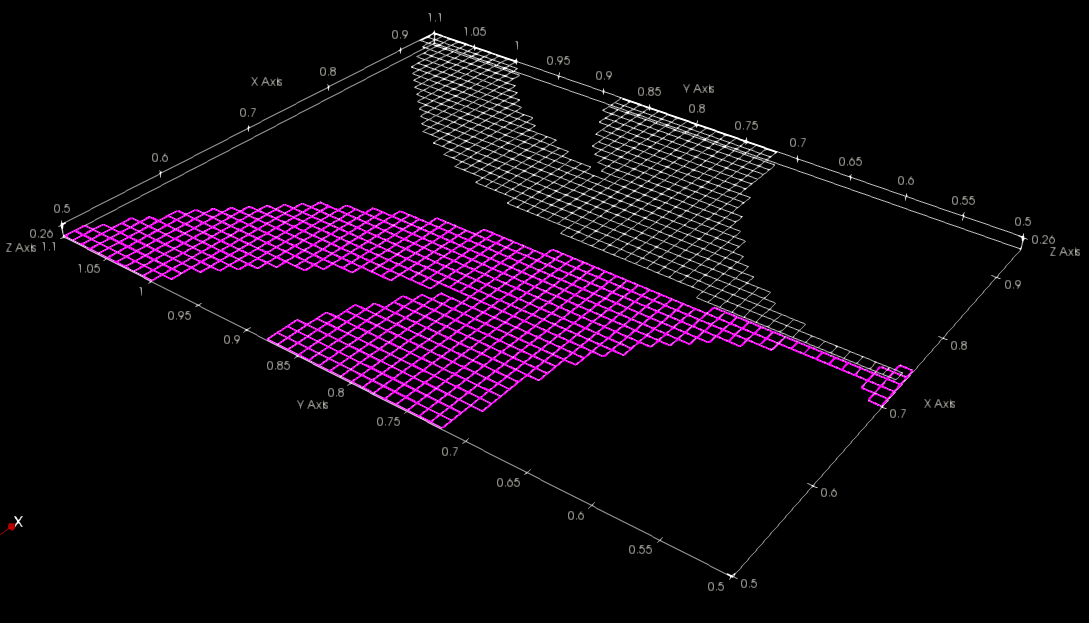
\includegraphics[width=0.8\textwidth]{vivaldi_fdtd_grid.png}
	\caption[]{维瓦尔第天线FDTD网格模型}
	\label{vivaldi_fdtd_grid}
\end{figure}

为了检验在FDTD网格中建模的天线的辐射特性在多大程度上符合实际天线的参数,在电源出加载一中心频率为500MHz的高斯脉冲,运行仿真并记录电源处的
场值,由此可计算出此天线的$S_{11}$参数。图\ref{vivaldi_s11_compare}给出了天线$S_{11}$参数的仿真与实测结果对比,其中实测结果由矢量网络分析仪
在微波暗室中测得。可以看出从0.6GHz以下,仿真曲线与实测曲线基本吻合,而这也包括了团队探地雷达的实际工作频率范围。0.6GHz以上与实测曲线出现的
较大偏离的原因是为了提高计算效率FDTD网格的尺寸设置为10mm,从而使波长短的高频部分出现了较大的误差。
\begin{figure}[htbp]
	\includegraphics[]{vivaldi_s11_compare.pdf}
	\caption[]{维瓦尔第天线$S_{11}$曲线比较}
	\label{vivaldi_s11_compare}
\end{figure}

图\ref{vivaldi_propagation}给出了信号源能量在向外传播过程中某时刻的电场值分布图。可以看出天线有明显的方向性,
其辐射能量集中在天线的正前方,这也与天线的设计符合。
\begin{figure}[htbp]
	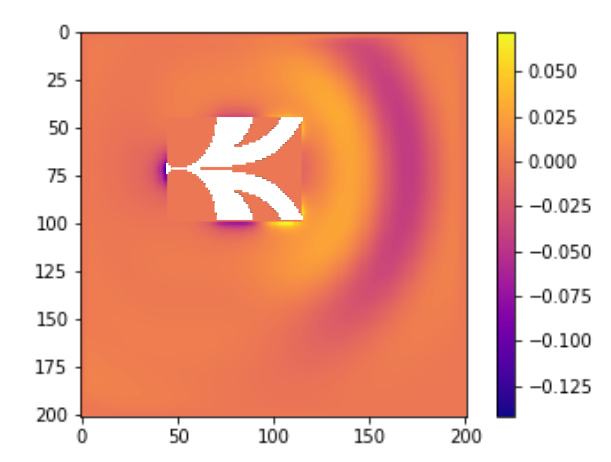
\includegraphics[width=0.8\textwidth]{vivaldi_propagation.png}
	\caption[]{维瓦尔第天线辐射电场值图}
	\label{vivaldi_propagation}
\end{figure}
\section{B 扫数据的批量生成}
利用gprMax结合前面实现的土壤模型和天线模型可以很方便地完成雷达回波数据的仿真。只需要定义好模型的几何尺寸和介质,信号源的频率和波形,以及
采集时间窗大小,就可以得到一道雷达回波。探地雷达在实际工作时一般会将天线在地面上沿水平移动并且按照一定的时间间隔记录一系列的波形,将这些
回波波形组合起来就可以得到雷达B扫图像。同样,在gprMax里也可以定义天线的移动的方向和间隔还有采集的回波数量,从而得到收发天线在模型内不同
位置的仿真结果,然后得到二维B扫图像。

如前所述,本章的目标是得到一系列的拟真B扫图像以供开发后面深度学习目标识别算法时使用。基于前面小节的内容,本节将介绍批量生成目标介质、位置、
大小和深度随机变化的B扫图像的过程。

gprMax 的建模是以文本形式的配置文件为基础的。在配置文件可以定义与仿真相关的参数,比如时间窗大小,介质参数,目标体大小等等。
配置文件里定义相关参数有命令法和脚本法两种。其中命令法最为基础,只要将相关建模命令的名称和参数直接组合起来
写在一行即可。比如\#domain 10 5 2就定义了整个仿真空间的大小为10x5x2米。脚本法比较灵活,可以通过函数调用
来使用建模命令,同时脚本法内还可以利用python语言控制极其复杂的建模操作,更重要的是命令法中需要手动写入
的参数在脚本法中都可以用变量代替,在修改模型某些几何参数时不用重新人工计算各个几何体的位置参数,
从而在复杂模型的构建时大大减小了出错的可能性。

利用脚本法可以满足构建本章介绍的复杂模型的需要。然而在批量生成仿真数据时,仿真模型内的目标参数在每次仿真时
都会发生变化,仅仅利用脚本法每次只能生成单一的模型。笔者在这里使用一个控制gprMax仿真的调度程序配合配置文件模板
来解决这一问题。配置文件模板和标准的gprMax配置文件格式一致,但是其中在每次仿真时需要随机变化的参数都以占位符
代替。调度程序本身也是一个python脚本,其功能是按照仿真需要生成符合预定范围的目标参数,然后将实际的目标参数
填写到配置文件模板里,最后调度程序将填写好的模板生成对应的配置文件并执行仿真。
这一流程可以用图\ref{gprmax_batch_model_procedure}描述。
\begin{figure}[htbp]
	\includegraphics[]{model_procedure.pdf}
	\caption[]{模型批量生成流程图}
	\label{gprmax_batch_model_procedure}
\end{figure}
\begin{figure}[htbp]
	\includegraphics[]{simu_chart.pdf}
	\caption[]{配置文件模板所对应模型剖面示意图}
	\label{simulation_chart}
\end{figure}

图\ref{simulation_chart}给出了本节所定义的配置文件模板所对应模型的剖面示意图。仿真空间长度为6m,宽度为1.5m,
高度为3m,网格尺寸为0.005m,PML层厚度为0.05m(10个网格);仿真空间的下半部分为拟真土壤模型,其中沙土与粘土所占
比例都是50\%,密度为$2g/cm^3$,含水量变化范围为0.1\%-2\%;天线离地面高度为0.2m,收发间距0.4m,天线起始位置
离模型的最左边0.5m,天线的移动总距离为4.6m,天线的移动步长为0.02m,总共采集230个位置的数据;信号源的波形为高斯脉冲,
中心频率为200MHz。

前面提到调度程序需要定义目标的参数范围。本文拟对地下目标的材质、位置、尺寸、深度等信息做识别,所以这里需要对
这些参数给定一个范围,让调度程序从中随机选择并生成B扫数据。
表\ref{table_geometry}给出了批量仿真时几何参数
范围;表\ref{table_material}给出了目标体可能的几种介质类型。
\begin{table}[htbp]
	\caption{目标体几何参数范围} 
	\begin{tabular}{|c|c|c|c|} 
		\hline  
		参数 &  最小值 & 最大值 \\
		\hline 
		水平坐标(m) & 2 & 4 \\  
		\hline  
		尺寸(m) & 0.1 & 0.3 \\  
		\hline  
		深度(m) & 0.1 & 0.4 \\  
		\hline  
	\end{tabular}
	\label{table_geometry}
\end{table}

\begin{table}[htbp]
	\caption{目标体介质类型} 
	\begin{tabular}{|c|c|c|c|} 
		\hline  
		介质 &  相对介电常数 & 电导率($S/m$)\\
		\hline 
		金属 & 10 & $10\times10^6$ \\  
		\hline  
		岩石 & 8 & $1\times10^{-6}$ \\  
		\hline  
		水 & 80 & $1\times10^{-6}$ \\  
		\hline  
	\end{tabular}
	\label{table_material}
\end{table}

定义好配置文件模板和调度程序中的参数范围便可以用来批量生成模型和对应的B扫数据。笔者在研究过程中
共自动生成了100个模型和B扫数据。图\ref{model_example}给出了其中两个模型的三维可视化结果。图
\ref{model_example}(a)的中的目标材质为金属,水平位置为3.6m,尺寸为0.18m,深度为0.33m;
图\ref{model_example}(b)的中的目标材质为岩石,水平位置为2.68m,尺寸为0.12m,深度为0.36m。

图\ref{bscan_example}给出了与图\ref{model_example}中的两个模型对应的仿真结果(已经过去背景处理)。
可以看到地面反射由于地面的起伏有较大的抖动。
\begin{figure}[H]
	\subfigure[]{
		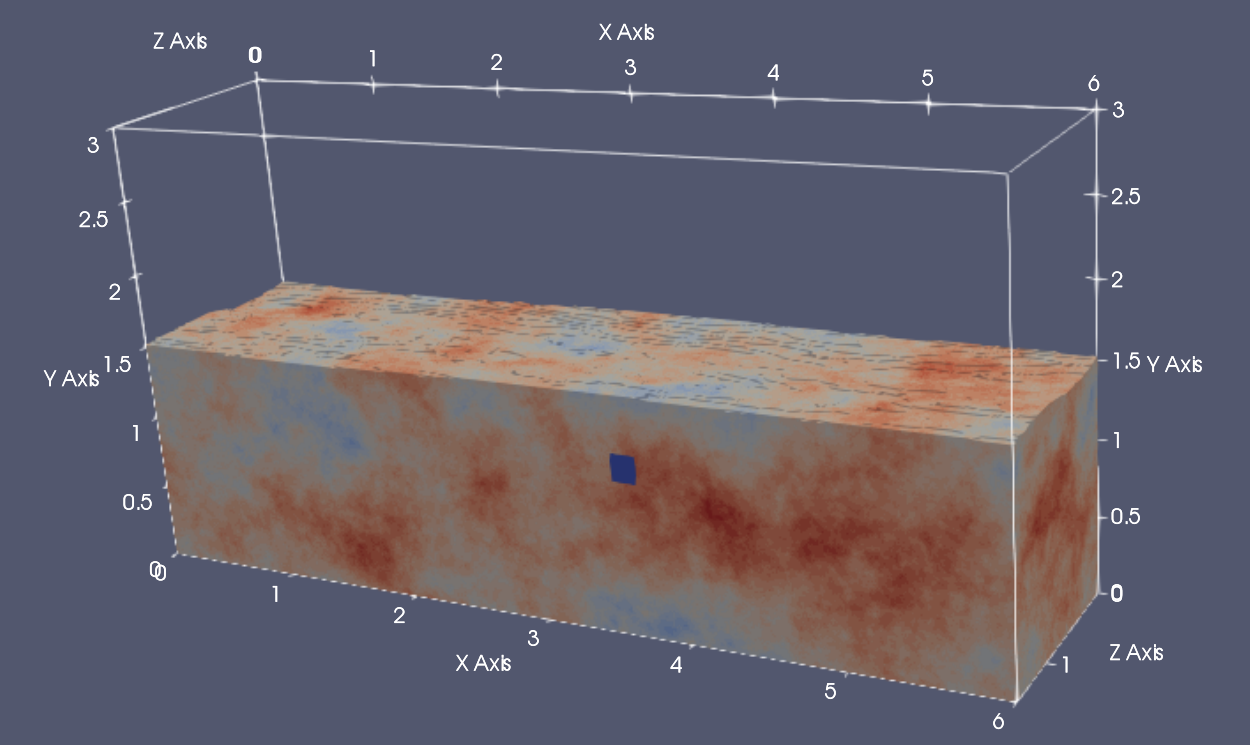
\includegraphics[width=0.8\textwidth]{model4.png}}
	\subfigure[]{
		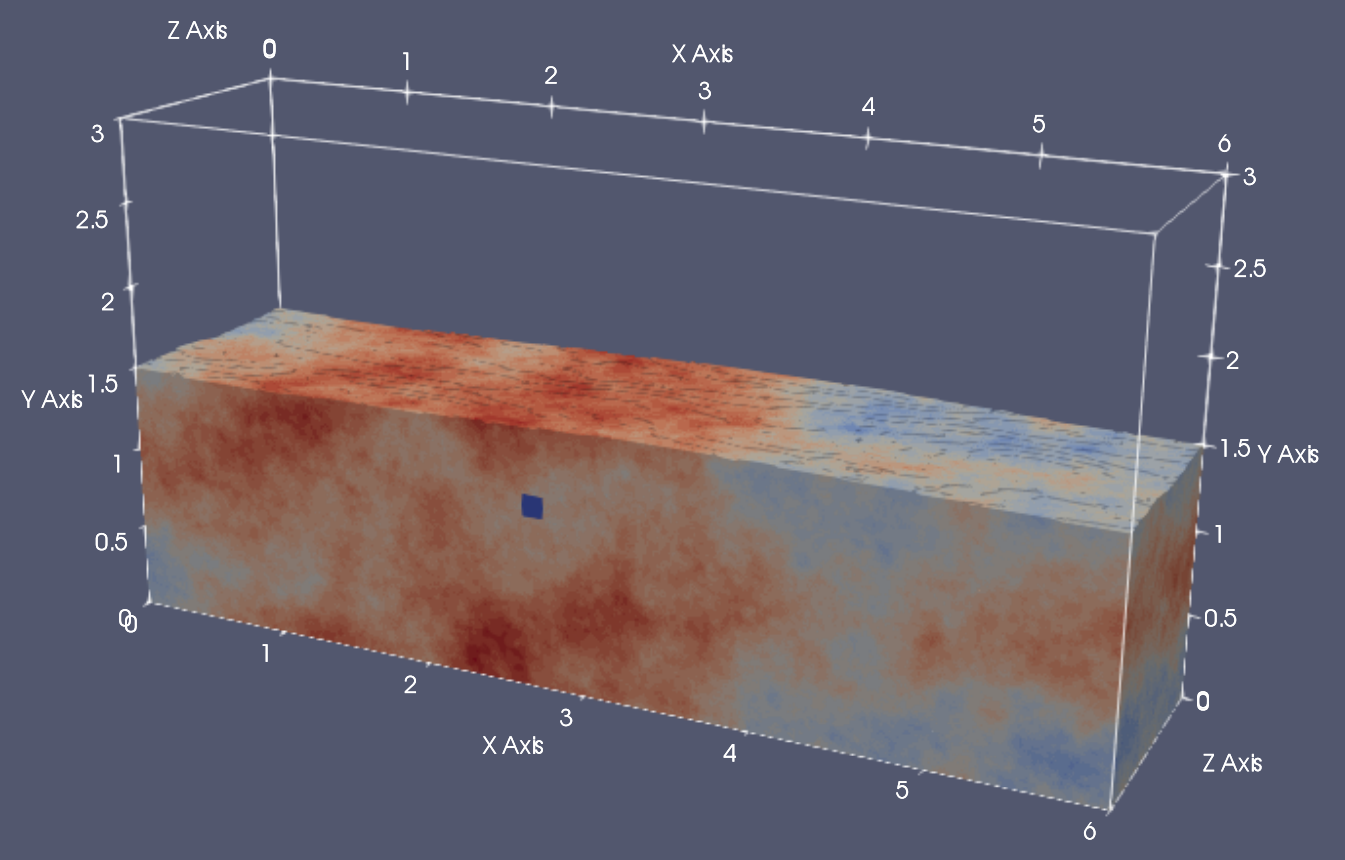
\includegraphics[width=0.8\textwidth]{model5.png}
	}
	\caption{随机模型示例}
	\label{model_example}
\end{figure}

\begin{figure}[H]
	\subfigure[]{
		\includegraphics[]{bscan4.pdf}}
	\subfigure[]{
		\includegraphics[]{bscan5.pdf}
	}
	\caption{批量生成的B扫示例}
	\label{bscan_example}
\end{figure}
\section{本章小结}
本章介绍了FDTD仿真的基本原理和开源数值仿真平台gprMax并
基于土壤介质参数半经验模型和FFT分形数据生成算法形成真实土
壤模型构建方法;针对模拟天线传输特征的问题,研究将真实天线几何模型内置到FDTD网
格的方法。最后结合配置文件模板和调度程序批量得到拟真雷达B扫图像。
\chapter{基于卷积神经网络的目标识别研究}
前面两章介绍深度学习的理论基础和地下目标仿真技术,本节将在这两章的基础上对仿真数据和实测数据实现
基于深度卷积网络的目标识别。主要内容包括:数据的预处理过程,网络模型的设计和训练,结果分析等。
\section{在仿真数据上的研究}
首先从数学上对本节的问题进行描述。设第三章所得到的B扫数据为一系列尺寸为$w\times h$的二维矩阵
$\mathbf{A}_i(i = 1...N)$,其中$N$代表所生成
B扫的总数量,$w$表示每道回波的采样点数,$h$表示每个B扫中所包含的波形道数。
对于每一个B扫$\mathbf{A_i}$,还可以设$m_i$、$p_i$、$s_i$、$d_i$分别为其建模时设定的目标材质、
目标水平位置、目标尺寸和目标深度。目标材质$m_i$为取值范围是0到3的整数,分别代表“无目标”、“岩石”,
“水”,“金属”这几种情况。本节的目的就是设计并训练深度神经网络使其对于给定的$\mathbf{A_i}$可以
较为近似地输出$m_i$、$p_i$、$s_i$、$d_i$的预测值$m_i^{\prime}$、$p_i^{\prime}$、$s_i^{\prime}$、
$d_i^{\prime}$。

就如何预测这四个值的问题,笔者做如下考虑。目标材质$m_i$是一个只有四种取值的离散值,所以对于材质
的预测是一个典型的分类问题,可以尝试用多层卷积网络辅之以softmax分类器解决。而$p_i$、$s_i$和$d_i$
的取值都是一个连续的实数,不能按常见的多分类问题处理。对于水平位置$p_i$和尺寸$s_i$,
可以联系到探地雷达数据的以下两个特点:第一,只有收发天线移动到目标附近时才会产生明显的反射信号;
第二,目标的尺寸将影响到B扫图像上反射信号的持续范围。基于这两个特点,可以设想若对于天线移动过程中的
所有位置均作材质预测,而不是对于整幅B扫图像作单一的预测,则可以利用材质预测的结果对目标水平位置和
尺寸做出判断。而对于深度值$d_i$,笔者拟采用处理回归问题的方法输出连续的预测值。
\subsection{数据预处理}
在设计和训练深度网络之前,首先必须准备好训练样本$\mathbf{X}_{train}$、训练样本标签$\mathbf{Y}_{train}$、
测试样本$\mathbf{X}_{test}$、测试样本标签$\mathbf{Y}_{test}$。由于在这里要对天线经过的每个位置均
做出材质预测,所以必然要对原始B扫数据做出切分处理,使得天线经过的每个位置都对应一小块B扫图像的子区域,
另外还需要在样本标签中设置对应这些子区域的标签向量来表示实际的材质。完整的数据切分过程如下:

1. 定义图像子区域的尺寸为$w_{sub}\times h$,天线每次移动距离为$d_{antenna}$,其中$w_{sub}$为子区域的宽度,其值大致等于B扫图像中双曲线
图案宽度的一半。

2. 设训练样本由$\mathbf{A}_1$...$\mathbf{A}_{N^{\prime}}$产生,
训练样本由$\mathbf{A}_{N^{\prime} + 1}$...$\mathbf{A}_{N}$产生,
则训练和测试样本按如下公式产生:
\begin{equation}
	\begin{aligned}
	\mathbf{X_{train}}[k] &= \mathbf{A}_i[x_{start}:x_{start} + w_{sub}]\qquad (i = 1...N^{\prime})\\
	\mathbf{X_{test}}[k] &= \mathbf{A}_i[x_{start}:x_{start} + w_{sub}]\qquad (i = N^{\prime} + 1...N)
	\end{aligned}
\end{equation}
其中$i = 1...N$,$x_{start} = 1...w - w_{sub}$,$k = 1 ... i \times (w-w_{sub})$;符号$A[a:b]$代表从$a$行
到$b$取子矩阵。

3. 训练样本标签和测试样本标签由收发天线中心到目标物水平位置的距离是否小于目标尺寸的两倍确定,写成公式形式为:
$$
\mathbf{Y}[i] = 
	\begin{cases} 
		onehot(m_i) & |(x_{start} + w_{sub} / 2 - \frac{p_i}{d_{antenna}}| \leq \frac{2 s_i}{d_{antenna}} \\
		onehot(1)   & Others
	\end{cases}
$$
其中$onehot(m_i)$函数表示将介质类型所对应的整数转化为对应的四阶向量形式,即$onehot(1)=[1\quad 0 \quad 0 \quad 0]$,
$onehot(2)=[0\quad 1 \quad 0 \quad 0]$...$onehot(4)=[0\quad 0 \quad 0 \quad 1]$。
\begin{figure}[htbp]
	\includegraphics{bscan_slice.pdf}
	\caption[]{B扫数据切分示意图}
	\label{bscan_slice}
\end{figure}

图\ref{bscan_slice}为数据切分过程的示意图。图中的B扫图像对应的是某金属目标的图像,所以在目标附近的子图像对应的
标签为[0 0 0 1],而远离目标的子图像对应的标签为[1 0 0 0],表示无目标。

接下来还需要对样本数据进行更进一步的处理,分别是时间子采样和归一化。进行时间子采样的原因是雷达B扫数据特别是仿真得出
的B扫数据往往在时间方向上的数据点数$w$比行进距离方向的数据点数$h$多一个量级以上,这样既会导致数据量太大影响
训练速率也会导致切分后的子图像的纵横比过大而导致矩形卷积核无法图像上的目标特征,因此在不影响图像本来形态的情况下
可以对原始数据在时间方向上做子采样处理,使纵横比大致处于一个量级。而归一化操作的目的是使所有数据的值限定在[0, 1]范围
内,从而使所有的样本都处于同一量级,避免奇异样本的影响。

时间子采样处理的数学表达为:
\begin{equation}
	\mathbf{A}^{\prime}_i[m, n] = \mathbf{A}_i[m, t_{sample} n] \qquad
	 (i = 1...N, m = 1...h, n = 1...[\frac{w}{t_{sample}}]) 
\end{equation}

常见归一化方法为最大最小归一化,其数学表达式为:
\begin{equation}
	\mathbf{X}_i^{\prime}=\frac{\mathbf{X}_i-\min (\mathbf{X}_i)}
	{\max (\mathbf{X}_i)-\min (\mathbf{X}_i)}
\end{equation}

经过前面的处理,第三章的100幅B扫数据被处理为17820道数据,其中各类型的样本数量如表\ref{table_sample_kind_unbalanced}所示。
\begin{table}[h]
	\caption{各类型样本数量} 
	\begin{tabular}{|c|c|c|} 
		\hline  
		样本类型 &  数量\\
		\hline 
		无目标 & 13385 \\  
		\hline  
		岩石 & 1507 \\  
		\hline  
		水 & 1142\\
		\hline
		金属 & 1386 \\
		\hline  
	\end{tabular}
	\label{table_sample_kind_unbalanced}
\end{table}

可以看出四种类型的样本中,岩石、水和金属的样本数量大致相等而无目标样本的数量远远大于其他类型,这样会导致
样本不平行的问题,从而影响后面深度神经网络的训练结果。为了解决这个问题可以在无目标样本中剔除部分数据,
使其剩余数量等于其他三类样本数量的平均值。

\subsection{网络结构设计与训练}
本节将设计和训练两个相互联系的深度卷积网络,分别称为“分类网络”和“回归网络”。其中,分类网络主要
解决的问题是对切分后子图像的目标材质的识别。而水平位置和尺寸的预测也可根据分类网络的输出结果
间接获得。和分类网络输出一个离散的分类结果不一样,回归网络的输出结果是一个实数,它的作用是对目标的
深度进行预测。
\subsubsection{分类网络}
本节所设计的网络结构以图\ref{cnn_structure}所示的卷积神经网络为基础,而具体的各层参数经过不断地试验尝试,
得到反复改进,最终形成了如表\ref{table_network_structure}所示的网络结构。
\begin{table}[h]
	\caption{地下目标识别神经网络结构} 
	\begin{tabular}{|c|c|c|} 
		\hline  
		层数 &  类型 & 参数\\
		\hline 
		1 & 卷积层 & 32个$3\times 5$的核;relu激活\\  
		\hline  
		2 & Dropout层 & 丢弃率:0.25\\
		\hline
		3 & 汇聚层 & $2\times 2$最大汇聚\\
		\hline
		4 & 卷积层 & 64个$3\times 5$的核;relu激活\\  
		\hline  
		5 & Dropout层 & 丢弃率:0.25\\
		\hline
		6 & 汇聚层 & $2\times 2$最大汇聚\\
		\hline
		7 & 卷积层 & 128个$3\times 5$的核;relu激活\\
		\hline  
		8 & Dropout层 & 丢弃率:0.25\\
		\hline
		9 & 卷积层 & 128个$3\times 5$的核;relu激活\\
		\hline  
		10 & Dropout层 & 丢弃率:0.25\\
		\hline
		11 & 卷积层 & 128个$3\times 5$的核;relu激活\\
		\hline  
		12 & Dropout层 & 丢弃率:0.25\\
		\hline
		13 & 卷积层 & 128个$3\times 5$的核;relu激活\\
		\hline  
		14 & Dropout层 & 丢弃率:0.25\\
		\hline
		15 & 全连接层 & 神经元数量:4;激活函数:softmax\\
		\hline  
	\end{tabular}
	\label{table_network_structure}
\end{table}

此网络共使用了6层卷积结构,在每个卷积网络层之后均使用了Dropout层。根据文献\cite{srivastava2014dropout},
Dropout层的作用是缓解深度神经网络常出现
的过拟合问题。所谓过拟合,就是指在有限的数据上拟合了过于复杂的模型,从而使模型学习了数据上过于细节的特征。
过拟合会使模型在新数据上的泛化能力不够。将多个模型组合起来也能被用来减轻过拟合的问题,但是这种方法需要
消耗很多的模型训练时间。Dropout层在减轻过拟合方面不需要额外的计算消耗而且效果明显,其基本思路是在训练过程中
随机选择一些神经元并将它们以及它们与前后层之间的连接从网络中暂时删除,其作用相当于在训练过程中引入噪声和稀疏性
并迫使网络学习到数据中更加高阶的结构。

模型中各卷积层的尺寸设置为$3\times 5$,这是因为输入数据的形状基本呈竖长条状($50\times 128$),为了更好地匹配
输入数据的维度,这里在保持卷积核较小的情况下应该尽量使其宽高比接近于输入数据的宽高比。

另外每个卷积层的卷积核数量,即特征图的数量,在使用汇聚层之后均成倍增加。比如从第四层到第七层卷积核数就从64
增加到了128。这样做的考虑是汇聚层的使用会使数据
丢失近一半的信息(图像的尺寸减半),所以应增加特征图数量来弥补这一问题。

此神经网络模型采用python机器学习库Keras实现,后端为 Tensorflow,训练所用硬件为GeForce GTX 1080 Ti显卡。在
batchsize 为 128 时每训练一轮所需时间为17秒。图\ref{loss_acc_curve}为训练50轮时的损失函数曲线和正确率曲线。
\begin{figure}[htbp]
	\subfigure[]{
		\includegraphics{loss_curve.pdf}
		\label{loss_curve}
	}
	\subfigure[]{
		\includegraphics{acc_curve.pdf}
		\label{acc_curve}
	}
	\caption{(a)损失函数曲线;(b)正确率曲线}
	\label{loss_acc_curve}
\end{figure}
\subsubsection{回归网络}
对于目标深度的预测不能传统的分类问题,而且深度的值也不能像尺寸和水平位置一样通过分类的结果间接得到,所以这里需要
另外设计一个网络来解决深度值的预测问题。

通过观察某B扫图像处于目标中心位置那道波形(图\ref{trace_above_object}),可以看出在5-10ns处存在强烈的直达波信号,而在15ns处
还可看到较弱的目标回波,若能训练一个可识别道波形中目标回波的神经网络则可解决深度的判定问题。
\begin{figure}[htbp]
	\includegraphics{trace_above_object.pdf}
	\caption{某B扫中位于目标中心处的波形}
	\label{trace_above_object}
\end{figure}

按照与表\ref{table_network_structure}类似的结构,笔者设计了一个卷积核宽度为1的深度卷积神经网络。这里将卷积核宽度设定
为1的原因是:与分类网络不同,此时的输入数据变成了一维波形,所以按照卷积核与输入数据匹配的原则其尺寸也要做相应调整。
表\ref{table_regression_structure}给出了此网络的结构。
\begin{table}[h]
	\caption{地下目标识别神经网络结构} 
	\begin{tabular}{|c|c|c|} 
		\hline  
		层数 &  类型 & 参数\\
		\hline 
		1 & 卷积层 & 32个$7\times 1$的核;relu激活\\  
		\hline
		2 & 卷积层 & 64个$7\times 1$的核;relu激活\\  
		\hline
		3 & 卷积层 & 128个$7\times 1$的核;relu激活\\
		\hline
		4 & 全连接层 & 神经元数量:32;relu激活\\
		\hline
		5 & 全连接层 & 神经元数量:64;relu激活\\
		\hline
		6 & 全连接层 & 神经元数量:1;relu激活\\
		\hline  
	\end{tabular}
	\label{table_regression_structure}
\end{table}

这里还需注意的是,回归网络的输出层不再是分类网络中用到softmax层,而是一个只有一共神经元的全连接层,这是因为
回归网络并不需要输出每个分类可能的概率,而仅仅需要输出一连续的实数作为深度的预测结果。
\subsection{结果分析}
为了直观地展示上节神经网络的预测结果,图\ref{material_prediction}给出了某幅测试样本中的B扫在
相同的横坐标下目标介质识别问题的预测结果和实际结果,底部的B扫图像可作为预测结果的参照。
\begin{figure}[htbp]
	\includegraphics{material_prediction_80.pdf}
	\caption[]{预测结果与B扫对比图}
	\label{material_prediction}
\end{figure}

可以看出对于该测试B扫,预测曲线和实际曲线高度吻合,目标的性质岩石识别正确,仅在目标左侧预测曲线的范围略微
超出实际曲线的范围。按照4.2.1节的讨论,其中所使用的图像切分使得预测结果与天线位置信息相关,
实际曲线中位于目标位置上方的矩形窗的宽度也与目标的尺寸相关。所以利用介质类别的预测结果曲线,也可以间接
对目标的水平位置和尺寸做出预测。

设某幅B扫图像$\mathbf{A}_i$预测曲线为取值为0到4的一维整数数组$\mathbf{P}$,其值分别对应无目标、岩石、水和金属这几种
情况。对于整幅B扫图像,介质种类的预测结果$m_i^{\prime}$可由$\mathbf{P}$中的最大值$max(\mathbf{P})$来表示。而
介质的水平位置可用矩形窗的中心来计算,即:
\begin{equation}
	p_i^{\prime} = mean(nonzero(\mathbf{P}))\times d_{antenna}
\end{equation}
其中函数$nonzero$表示求解数组中非零元素的下标,函数$mean$用来求解平均数。

目标尺寸的预测结果$s_i^{\prime}$的计算方法为:
\begin{equation}
	s_i^{\prime} = \frac{1}{4 p_i^{\prime}}\sum{\mathbf{P}}\times d_{antenna}
\end{equation}

图\ref{material_bar}绘出了在测试B扫数据上目标材质$m_i$与$m_i^{\prime}$的详细对比结果,可以看到除了第13组所有
测试B扫均预测正确,综合正确率为95\%。
\begin{figure}[htbp]
	\includegraphics{material_bar.pdf}
	\caption[]{目标材质预测结果}
	\label{material_bar}
\end{figure}

图\ref{position_bar}给出了在测试B扫数据上目标水平位置的预测结果。经计算,水平位置预测的平均相对误差为2.3\%。
\begin{figure}[htbp]		
	\includegraphics{position_bar.pdf}
	\caption[]{目标水平位置预测结果}
	\label{position_bar}
\end{figure}

图\ref{size_bar}给出了在测试B扫数据上目标水平位置的预测结果。目次尺寸预测的平均相对误差为8.1\%。
\begin{figure}[htbp]
	\includegraphics{size_bar.pdf}
	\caption[]{目标尺寸预测结果}
	\label{size_bar}
\end{figure}
\section{在实验数据上的研究}
为了验证前述深度网络在实测雷达B扫数据上的效果,本节采用某次在沙坑进行的探地雷达金属地雷目标探测实验的数据并尝试
对目标的所在位置进行识别。
\subsection{实验情况介绍}
现场实验使用自行开发的超宽带(UWB)GPR系统\citing{huo2014design}进行。该系统由发射器,天线,接收器,数据采集板和安装有控制软件的PC机组成。超宽带电磁脉冲通过第三章所述Vivaldi天线由双极性高斯脉冲源辐射,工作频率为210MHz,最大电压为830V。然后,反射信号由另一个天线接收并传送到数据采集板。信号在数据采集板中进行采样和数字化,并通过串口传输到pc软件。 2D扫描图像和其他系统指标在PC软件上实时显示。
\begin{figure}[htbp]
	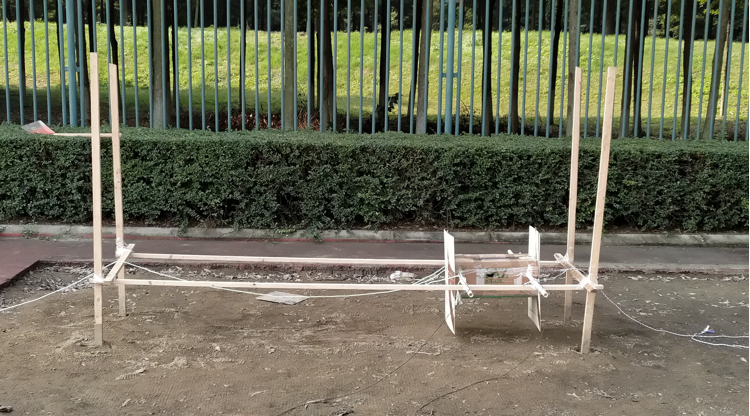
\includegraphics{sandpit_photo.png}
	\caption[]{沙坑实验现场}
	\label{sandpit_photo}
\end{figure}

实验场地位于电子科技大学清水河校区体育场的跳远沙坑中(图\ref{sandpit_photo})。该测试旨在检测非实验室环境中的地雷。实验在雨后两天进行,以确保土壤中适当的含水量。土壤含水量高会导致电磁波强烈衰减,因此难以成功探测到地雷。沙坑表面呈起伏状,大致起伏范围为-1.5cm到+1.5cm。
\begin{figure}[htbp]
	\includegraphics{sandpit_model.pdf}
	\caption[]{沙坑实验示意图}
	\label{sandpit_model}
\end{figure}

实验使用木架搭建了一个简易滑轨,滑轨长3米,收发天线被固定在纸箱两侧并可沿着水平木架行进(图\ref{sandpit_model})。实验时,收发天线可由固定在两侧的绳子来回拉动。

由于没有实际的地雷,所以用某个$10\times 10$cm的铁板来代替。实验期间一共收集了7组雷达B扫数据。
第一组实验时沙坑内没有填埋任何物体。在进行第2组到第6组实验时,铁板分别填埋在图\ref{sandpit_model}中所标识的A-E处。第7组实验时,铁板放置在位置F处,并将塑料瓶埋入50厘米远的地方作为干扰物。1到6组数据用作训练样本。跟踪组7是测试数据。进行每组实验时,天线都会在木架上被来回拉动20次,所以实验共取得140道雷达B扫数据。
\subsection{数据预处理}
本章前面小节建立的数据切分方案完全可以直接用到实测数据的处理上,所以具体的预处理过程不再赘述。在这里只需要注意几个问题:

1. 本次实验中由于不涉及分类问题,所以在这里标签不再是长度为4的向量,而是长度为2的向量,且可能的取值为
[1 0]或者[0 1],分别用来代表当前位置有目标和当前位置没有目标。

2. 本次实验标签无法通过计算机程序直接计算得出,而是需要根据现场的实验记录人工标注。

通过切分处理,最后共得到7266组训练样本和1038组测试样本。
\subsection{网络训练和结果分析}
\begin{figure}[htbp]
	\includegraphics{sandpit_result.pdf}
	\caption[]{沙坑实验结果示例}
	\label{sandpit_result}
\end{figure}

\begin{table}[h]
	\caption{各类型样本数量} 
	\begin{tabular}{|c|c|c|} 
		\hline  
		正确率 & 虚警率 & 漏报率\\
		\hline
		94.2\% & 3.9\% & 1.9\%\\
		\hline
	\end{tabular}
	\label{table_sanpit_acc}
\end{table}
\section{本章小结}
 
\chapter{全文总结与展望}

\section{全文总结}
本文以探地雷达地下目标识别这个问题为背景,针对目前传统算法需要大量的人工干预和专业知识
的局限性,并结合探地雷达B扫数据和光学图像的相似性,使用深度学习技术来解决地下目标
识别的问题。本文在近年来国内外机器学习在地下目标识别的研究工作的基础上,不仅做到了
对地下目标有无的识别,还发展出了对地下目标介质、尺寸、深度等信息的识别方法。本文所形成的
目标识别方法最终在仿真数据和实测数据上均得到验证。

概括来说本文研究过程中主要解决的问题是:

1. 在构建拟真土壤模型时。查阅前人关于土壤的组成和含水率对复介电常数的影响的研究成果,
并将其与分形特征数据生成算法相结合,形成拟真土壤模型的建模方法。

2. 在天线建模与模型批量生成方法研究过程中。研究python语言在探地雷达地下目标识别建模领域
的应用原理,形成一套自动化地下目标仿真程序。

3. 在构建深度网络模型时。形成一组合适的B扫数据的预处理流程。比较各种参数和网络结构对识别效果
的影响,并在最后得到准确率优秀的网络模型。

\section{后续工作展望}
深度学习领域在最近几年发展迅速。2018年,关于深度学习在电磁探测领域的研究的文献更是相继出现。
在本文研究工作的基础上,后续工作可在以下几个方面继续展开:

1. 本文在仿真数据上实现了对地下目标材质、位置、深度、尺寸等信息的识别,但是由于实验条件所限,
在实验数据上并没有来得及对材质深度等信息的识别进行验证。所以下一步的工作首先可就本文的方法在
实验数据上的全面验证上展开。

2. 本文在进行天线建模过程中,由于整个FDTD网格的空间步长是一致的,所以在对天线几何模型的细节处理方面
存在妥协,因而影响了天线仿真的精度。若使用次网格等技术,则有望实现在模型细节之处对FDTD网格进一步局部剖分,
解决模型精度与计算速度之间的矛盾。
\chapter{template}
This is the template of the chapter in split file.

\section{s1}
This is a section.

\subsection{sub1}
This is a subsection.

% misc

\thesisacknowledgement
在攻读博士学位期间,首先衷心感谢我的导师XXX教授

\thesisloadbibliography[nocite]{reference}

%
% Uncomment following codes to load bibliography database with native
% \bibliography command.
%
% \nocite{*}
% \bibliographystyle{thesis-uestc}
% \bibliography{reference}
%

% comment while no need
%
\thesisappendix


\thesisloadachievement{publications}
%
\thesistranslationoriginal
\section{The OFDM Model of Multiple Carrier Waves}


%
\thesistranslationchinese
\section{基于多载波索引键控的正交频分多路复用系统模型}



\end{document}
